\section{Development}
\subsection{Initial function}
This section concerns getting the tracker to the point where it can transmit \acrshort{gps} location 
via \gls{lora}.
\subsubsection{Hardware}
The Feather (M0 \gls{lora}) and \acrshort{gps} Featherwing are designed to
be directly stackable\footnote{
    \Cref{fig:gpstack}.
}, and as such share the same pin placement and 2D dimensions. 
The pinout diagram for the Feather M0 can be found 
in \cref{fig:m0pinout}, with matching pin placement for the \acrshort{gps} Featherwing 
in \cref{fig:gpspin}.

Therefore, each pin can be soldered directly using included headers.
For now, additional hardware like batteries and antennae are not necessary, as only
basic function will be tested. 

The Pi \acrshort{hat} is similarly configured to slot onto the \acrshort{gpio} pins
available on the Pi 3 directly. Pinout diagrams for the board can be 
found in \cref{fig:raspipinout}. No additional work is required to interface the hardware.

\subsubsection{\acrshort{gps}}
\label{sec:devgps}
With the boards soldered together, basic operation can be checked 
by loading the `blink' sketch \cite{arduino:blink} using Arduino's \acrshort{ide}.
This sketch will simply switch the inbuilt LED on and off every second, and can be used to verify that
the board can accept and run sketches.

\begin{wrapfigure}[11]{R}{0.6\textwidth}
    \vspace{-5pt}
    \centering
    \captionsetup{justification=centering}
    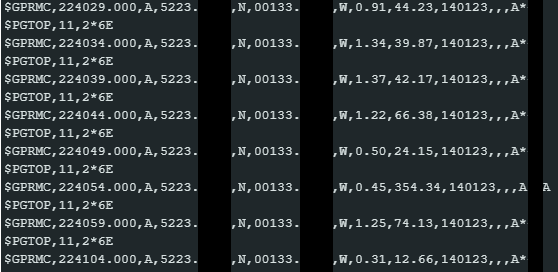
\includegraphics[width=0.6\textwidth]{../figures/hardwareserialoutput.png}
    \caption[GPS hardware serial output]{\acrshort{gps} hardware serial output with sensitive location data censored,
        showing \gls{gprmc} and \gls{pgtop} sentences.}
    \label{fig:gpshardwareserial}
\end{wrapfigure}


Having proven basic function, the next test concerns the function of the specific hardware. The \acrshort{gps} module
will be focused on to begin with.

The initial test sketch as per the documentation \cite{adafruit:gps, adafruit:gpshardwareserial} is loaded.
This produces output as in \cref{fig:gpshardwareserial}.
% \begin{figure}[H]
%     \centering
%     \captionsetup{justification=centering}
%     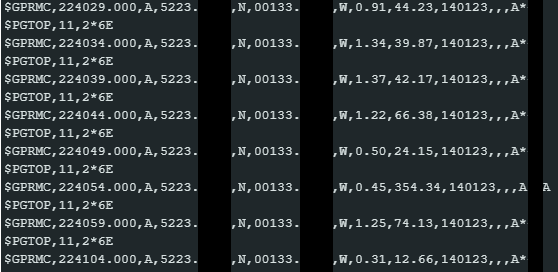
\includegraphics[width=0.5\textwidth]{../figures/hardwareserialoutput.png}
%     \caption[GPS hardware serial output]{\acrshort{gps} hardware serial output with sensitive location data censored,
%         showing \gls{gprmc} and \gls{pgtop} sentences.}
%     \label{fig:gpshardwareserial}
% \end{figure}

By default, the \acrshort{gps} module outputs many standardised \acrshort{nmea} sentences,
the most important of which to begin with is the \gls{gprmc} sentence.

\begin{lstlisting}[label=code:gprmcsentence, caption={\acrshort{nmea} \gls{gprmc} sentence example},captionpos=b]
$GPRMC,224029.000,A,5223.00,N,00133.00,W,0.91,44.23,140123,,,A*40
\end{lstlisting}

The output format is not immediately obvious. The \cref{code:gprmcsentence} can be broken down as follows \cite{baddeley:nmea, novatel:gprmc}:
\begin{description}[align=left, labelwidth=2.5cm,labelindent=1cm]
    \item[\gls{gprmc}] Message ID
    \item[223029.00] Time in UTC (22:30:29.00)
    \item[A] Validity - \textbf{A}ctive/\textbf{V}oid
    \item[5223.00,N] Latitude (52\textdegree23.00'' North\footnote{The longitude and latitude appear to be in
            decimal degrees at a glance and will therefore return errors when attempting to plot with this expectation.
            Furthermore, it is specifically degrees minutes and not degrees minutes seconds as one may expect.})
    \item[00133.00,W] Longitude (001\textdegree33.00'' West)
    \item[0.91] Speed (knots)
    \item[44.23] Tracking angle
    \item[140123] Date (14\textsuperscript{th} January 2023)
    \item[A] Positioning mode indicator 
        \begin{description}[align=left, labelwidth=1cm,labelindent=2.75cm]
            \item[A] Autonomous
            \item[D] Differential
            \item[E] Estimated (dead reckoning)
            \item[M] Manual input
            \item[N] Data not valid
        \end{description}
    \item[40] Checksum (XOR of all bytes between \$ and *)
\end{description}

The output location was verified to be correct. Obtaining a fix while indoors proved very difficult. The \acrshort{gps} module uses
coin cell to save fix data, which would have helped obtain a fix outdoors and then move indoors to observe the data.

The \gls{pgtop} sentence characterises the antenna connection, a non-standard command specific to the FGPMMOPA6H module \cite{gtop:pa6h}.
\begin{lstlisting}[label=code:pgtopsentence, caption={\acrshort{nmea} \gls{pgtop} sentence example},captionpos=b]
    $PGTOP,11,2*6E
\end{lstlisting}
\Cref{code:pgtopsentence} can be broken down as follows:
\begin{description}[align=left, labelwidth=2cm,labelindent=1cm]
    \item[\gls{pgtop}] Message ID
    \item[11] Command ID
    \item[2] Antenna status
        \begin{description}[align=left, labelwidth=0.75cm,labelindent=2.25cm]
            \item[1] Active antenna shorted
            \item[2] Using internal antenna
            \item[3] Using external (active) antenna
        \end{description}
    \item[6E] Checksum
\end{description}

The antenna status is not particularly useful, especially so at this stage of the development.
Therefore, it can be disabled. Many of the commands to program the device (for example,
changing the sentence output frequency) can be found in the \gls{pmtk} reference document\footnote{
    With a battery, the \gls{pmtk} commands are retained and do not
    need to be presented to the module on power-on. Otherwise, settings must be reconfigured on
    every boot.} \cite{gtop:pmtk}.
Alternatively, the Adafruit \acrshort{gps} library \cite{adafruit:gpslibrary} has support for some commands.
These commands are not documented and can only be found hardcoded into the header file of the
library \cite{adafruit:gpspmtk}.

Regarding the antenna, it can be disabled in two ways, via serial\footnote{This must be the serial
    connection to the \acrshort{gps} device from the main board, and cannot be accessed directly via serial monitor.
    In order to send commands on the fly via serial monitor, the code must be configured to then forward those commands
    to the correct serial connection (in the case of \cref{code:pgtopdisableserial}, `serial1').} :
\begin{lstlisting}[label=code:pgtopdisableserial, caption=\relax,captionpos=b]
    #define GPSSerial Serial1
    GPSSerial.println("$PGCMD,33,0*6D");
\end{lstlisting}
or using the library:
\begin{lstlisting}[label=code:pgtopdisablecmd, caption=\relax,captionpos=b]    
    Adafruit_GPS GPS(&GPSSerial);
    GPS.sendCommand(PGCMD_NOANTENNA);    
\end{lstlisting}

The library provides some useful functions and makes the code less verbose and more readable,
however it may prove to include significant enough overhead to impact the battery life.
If that happens to be the case the library can be removed as essential function
can be programmed to the \acrshort{gps} chip directly via serial.

\subsubsection{Pi \gls{lora}}
The \gls{lora} bonnet library as provided by Adafruit requires Circuit Python to be installed
on the Pi \cite{adafruit:circuitpython,adafruit:lorabonnet}\footnote{The installation documentation
    concerns both RFM69 and RFM9X radios. This project uses the RFM95W radio, also referred to
    as \gls{lora}.}.

With required software, libraries, and fonts installed, the example code \cite{adafruit:rfm95check}
can be loaded. This checks that the radio is present and the \acrshort{oled} displays correctly.

Finally, the radio function script can be loaded \cite{adafruit:radiopy}. This will await
incoming \gls{lora} packets, but can also send data using the buttons.

\subsubsection{Feather \gls{lora}}

\gls{lora} transmission with this board relies on the RadioHead library \cite{airspayce:main} in order to
transmit \gls{lora} packets, installation details for which can further be found in the
documentation \cite{adafruit:loram0}.

The transmission test script can be loaded onto the Feather \cite{adafruit:feathertx} once required software
has been installed. This will transmit a packet every second and await a reply.
For the time being, the Pi will not automatically send a reply, so the Feather will output
the ``error text''. This is of little consequence as the Pi
primarily only needs to work as a receiver with no two-way communication\footnote{The test script on the
    Pi does in fact allow output by pressing one of the buttons. This can be used to test communications
    and will be picked up by the Feather if this is tested.}.

\subsubsection{\gls{lora} with \acrshort{gps}}
With one-way communication working as expected\footnote{Both example scripts are set at \qty{915.00}{\MHz}
    and will work by default. This needs to be adjusted to \qty{868.00}{\MHz} for use in the UK
    \cite{ofcom:licenceexempt}.}, the next step is to integrate \gls{lora} with \acrshort{gps} on the Feather. This
stage is where communication collision issues have occurred in previous projects,
however as the \acrshort{gps} module uses the second serial connection and the \gls{lora} chip uses \acrshort{spi}, no such
issues should occur.

For streamlined testing, the library will be used to strip the data sent to only latitude, longitude, and packet number
(incremented every time \acrshort{gps} location is fixed to indicate that the location is up-to-date). The various
segments of data then need to be placed together in a structure. The public member function \lstinline{send()} of the
\lstinline{RH_RF95} class \cite{airspayce:docs} takes two arguments, \lstinline{data (uint8_t*)} and \lstinline{len (uint8_t)}.
This means that the data to be sent needs to be consolidated into a single structure, with the pointer to the structure
and its length sent to the function. The Arduino compiler is built on processing AVR-C and therefore suffers when handling
strings and performing conversion and concatenation natively, which can lead to complex and verbose code.
The Arduino \acrshort{ide} also supports C++ classes and function, amongst which
include the \lstinline{String} class and \lstinline{+} concatenating function
\cite{arduino:introduction, arduino:reference}. While the class may prove problematic on embedded hardware
due to memory fragmentation on the heap, for the time being it is sufficient where the primary goal is
functional and readable code. Two additional benefits are that the length is also easily attainable
as the method \lstinline{.length()} on the class, and also conversion to an array of type \lstinline{char} is supported.
\Cref{code:transmissionbody} shows a snippet of the body code.

\begin{lstlisting}[language=C++,label=code:transmissionbody,caption={Transmission body code},captionpos=b]
void loop() {
    //buffer gps location
    char c = GPS.read();           
    //interpret whether new location obtained and parse
    if (GPS.newNMEAreceived()) {    
        if (!GPS.parse(GPS.lastNMEA())) { 
            return;
        }
    }
    //execute every 5 seconds
    if (millis() - timer > 5000) {  
        timer = millis(); 
        //increment packet counter if new fix obtained
        if (GPS.fix) {
            count++;                
        }
        //produce concatenated string
        String output = String(count) + ": " + String(GPS.latitude,4) + "," + String(GPS.longitude,4);      
        length = output.length();
        //create variable send to hold packet once converted to type char
        char send[length];          
        output.toCharArray(send, length);
        Serial.println(send);   
        rf95.send((uint8_t *)send, length);        
    }
}
\end{lstlisting}

The output can be observed in \cref{fig:loraoutput}, showing \gls{lora} and GPS working together.

\begin{figure}[H]
    \label{fig:loraoutput}
    \begin{subfigure}{0.45\textwidth}
        \centering
        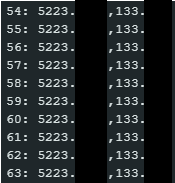
\includegraphics[height=4cm]{../figures/feather tx.png}
        \caption{Feather transmission logs}
    \end{subfigure}
    \hfill
    \begin{subfigure}{0.45\textwidth}
        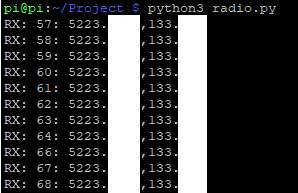
\includegraphics[height=4cm]{../figures/pi rx.png}
        \caption{Pi reception logs}
    \end{subfigure}
    \caption[LoRa communications with GPS location]{\gls{lora} communications with \acrshort{gps} location}
\end{figure}

\subsection{Power tester}
In order to determine the appropriate battery capacity to use, it is helpful to test the power consumption
of the transmitter over the expected period of use. Greater capacity batteries are heaver and larger - two
factors that need to be minimised. There is also the potential fire risk, however this is minimal without damage. 

By recommendation, a KCX-017 \acrshort{usb} tester was purchased to measure the current draw of the transmitter under
normal function. The included manual was poorly translated and difficult to follow, however a more
informative version was found online \cite{kcx}. No further details about the manufacturer or
any other products they may produce were found.

\subsubsection{Test specification}
\label{sec:powertestspec}
The outline of the test is to determine the appropriate battery required for the module. The tester
has various functions available, however only the capacity recording is relevant. The tester will
be plugged into a \acrshort{usb} outlet, and the transmitter will be plugged into the tester. The transmitter
will be plugged into the tester and will operate from thereon. Recordings will be taken every thirty
minutes for four hours as a preliminary measure of function. The Pi will be running to record
that the transmitter is operating as expected.

Two tests were performed:
\begin{enumerate}
    \item The transmitter was housed indoors so that it is unable to obtain a \acrshort{gps} lock. This
          will lead to the greatest power consumption.
    \item The transmitter was placed near a window so that it is able to update \acrshort{gps} location.
          This simulates normal operation.
\end{enumerate}

\paragraph{Risks}
The only identifiable risk is excessive current draw for the tester to handle. 
This risk is negligible as the tester is quoted to have a current limit 
of \qty{3500}{\mA} \cite{kcx},
which is far beyond the Feather capabilities. 

\subsubsection{Results}
Upon commencing the first test, the receiver registered no data. The cause was to simply
remove the line \lstinline{while (!Serial) delay(10);} as it prevents the code executing
until the serial interface is connected, so output can be monitored. In the case of this test,
serial output was not required, however the line still stalled the code.

With the change made and output occurring as expected, the meter did not appear to
register any changes. The meter was checked to be working by observing the current 
draw of a mobile phone, and was found to be operating as expected.
Thereafter, the meter was left and checked every hour.
The first change only occurred after three hours.

The consumption incremented only after three hours. It was left overnight and checked again,
at this point registering \qty{8}{\mAh}. The complete set of recordings
can be found in \cref{table:powermeter}. The data is plotted below using
code in \cref{script:powermeter}.
\begin{figure}[H]
    \centering
    \label{fig:powermeter}
    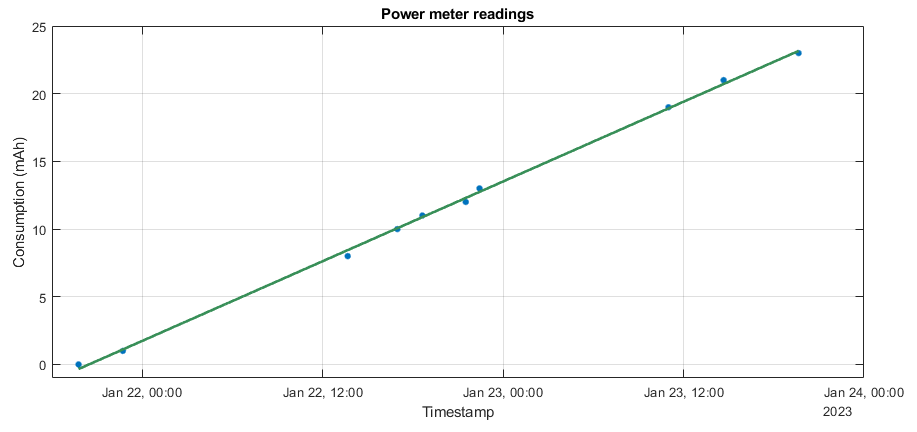
\includegraphics[width=\textwidth]{../../Tests/power meter/powermeter.png}
    \caption{Power meter results}
\end{figure}

The results suggest that, during normal operation, the transmitter requires around only
\qty{0.5}{\mA}. This is far too low to be accurate, and in turn,
likely means the meter does not have sufficient resolution
to measure the device. The meter does indicate a linear trend in power draw
suggesting predictability in normal use,
however given the poor accuracy of the data, the validity of this cannot be determined.

\subsection{Intermediate steps}
\label{sec:intermediate}
The power meter results were disappointing, however the documentation for the hardware
provides useful values with which an estimated battery capacity requirement can be produced.
The \gls{lora} board draws \qty{40}{\mA} when the radio is actively
listening, and draws \qty{130}{\mA} for \qty{70}{\ms} when transmitting at peak gain \cite{adafruit:loram0}.
The \acrshort{gps} module draws \qty{25}{\mA} when tracking and \qty{20}{\mA} during navigation \cite{adafruit:gps}.
This gives a rough total of \qty{60}{\mA} typical draw in the average case. Considering the
transmitter needs to operate for nine hours\footnote{\Cref{sec:specsbatt}.},
this suggests a battery capacity requirement of \qty{540}{\mAh}.

This suggests that a repurposed \qty{3.7}{\V}
\qty{500}{\mAh} quadcopter battery, may be used to test the transmitter functionality directly.
The \gls{lora} board requires a JST jack \cite{adafruit:loram0}. By investigating Adafruit's
other products, this appears to be a JST-PH connector specifically \cite{adafruit:jst}.

The battery header was removed and a JST-PH connector crimped onto the end of the leads.
The polarity was then checked before powering the transmitter and ensuring it functioned
as before.

\subsubsection{Code issues}
\label{sec:codeissues}
During such a function test, the code on the receiver end crashed twice, producing an error such
as in \cref{code:programerror}.

\begin{lstlisting}[caption={Program error message},label=code:programerror,captionpos=b]
Traceback (most recent call last):
    File "/radio.py", line 72, in <module>
        packet_text = str(prev_packet, "utf-8")
UnicodeDecodeError: 'utf-8' codec can't decode byte 0xae in position 0: invalid start byte
\end{lstlisting}

Due to the module being powered up and disconnected abruptly multiple times
while setting up the battery, the suspicion was that transmission was interrupted midway,
leading to the receiver attempting to parse an unfinished and corrupted packet. However,
given the time window of less than \qty{100}{\ms} for transmission, the fact this occurred
twice suggests this theory may not be likely.

In order to test how long the transmitter is able to function, the code needs to be
improved to be more resilient and stable. The example code \cite{adafruit:radiopy} has
been updated to safely handle the exception. While the cause of the error has not been
determined or investigated further at this point, the code will now attempt to parse
the packet in a \lstinline{try/except} block. The first handles the
\lstinline{UnicodeDecodeError} directly, while the second handles anything else that
may occur, in case there are other issues that have not been uncovered. It will indicate
that an unexpected error has occurred and continue execution from thereon.
The modified code can be found in \cref{pi:radio}.

\subsubsection{Antenna}

\begin{wrapfigure}{R}{0.4\textwidth}
    \centering
    % \captionsetup{justification=centering}
    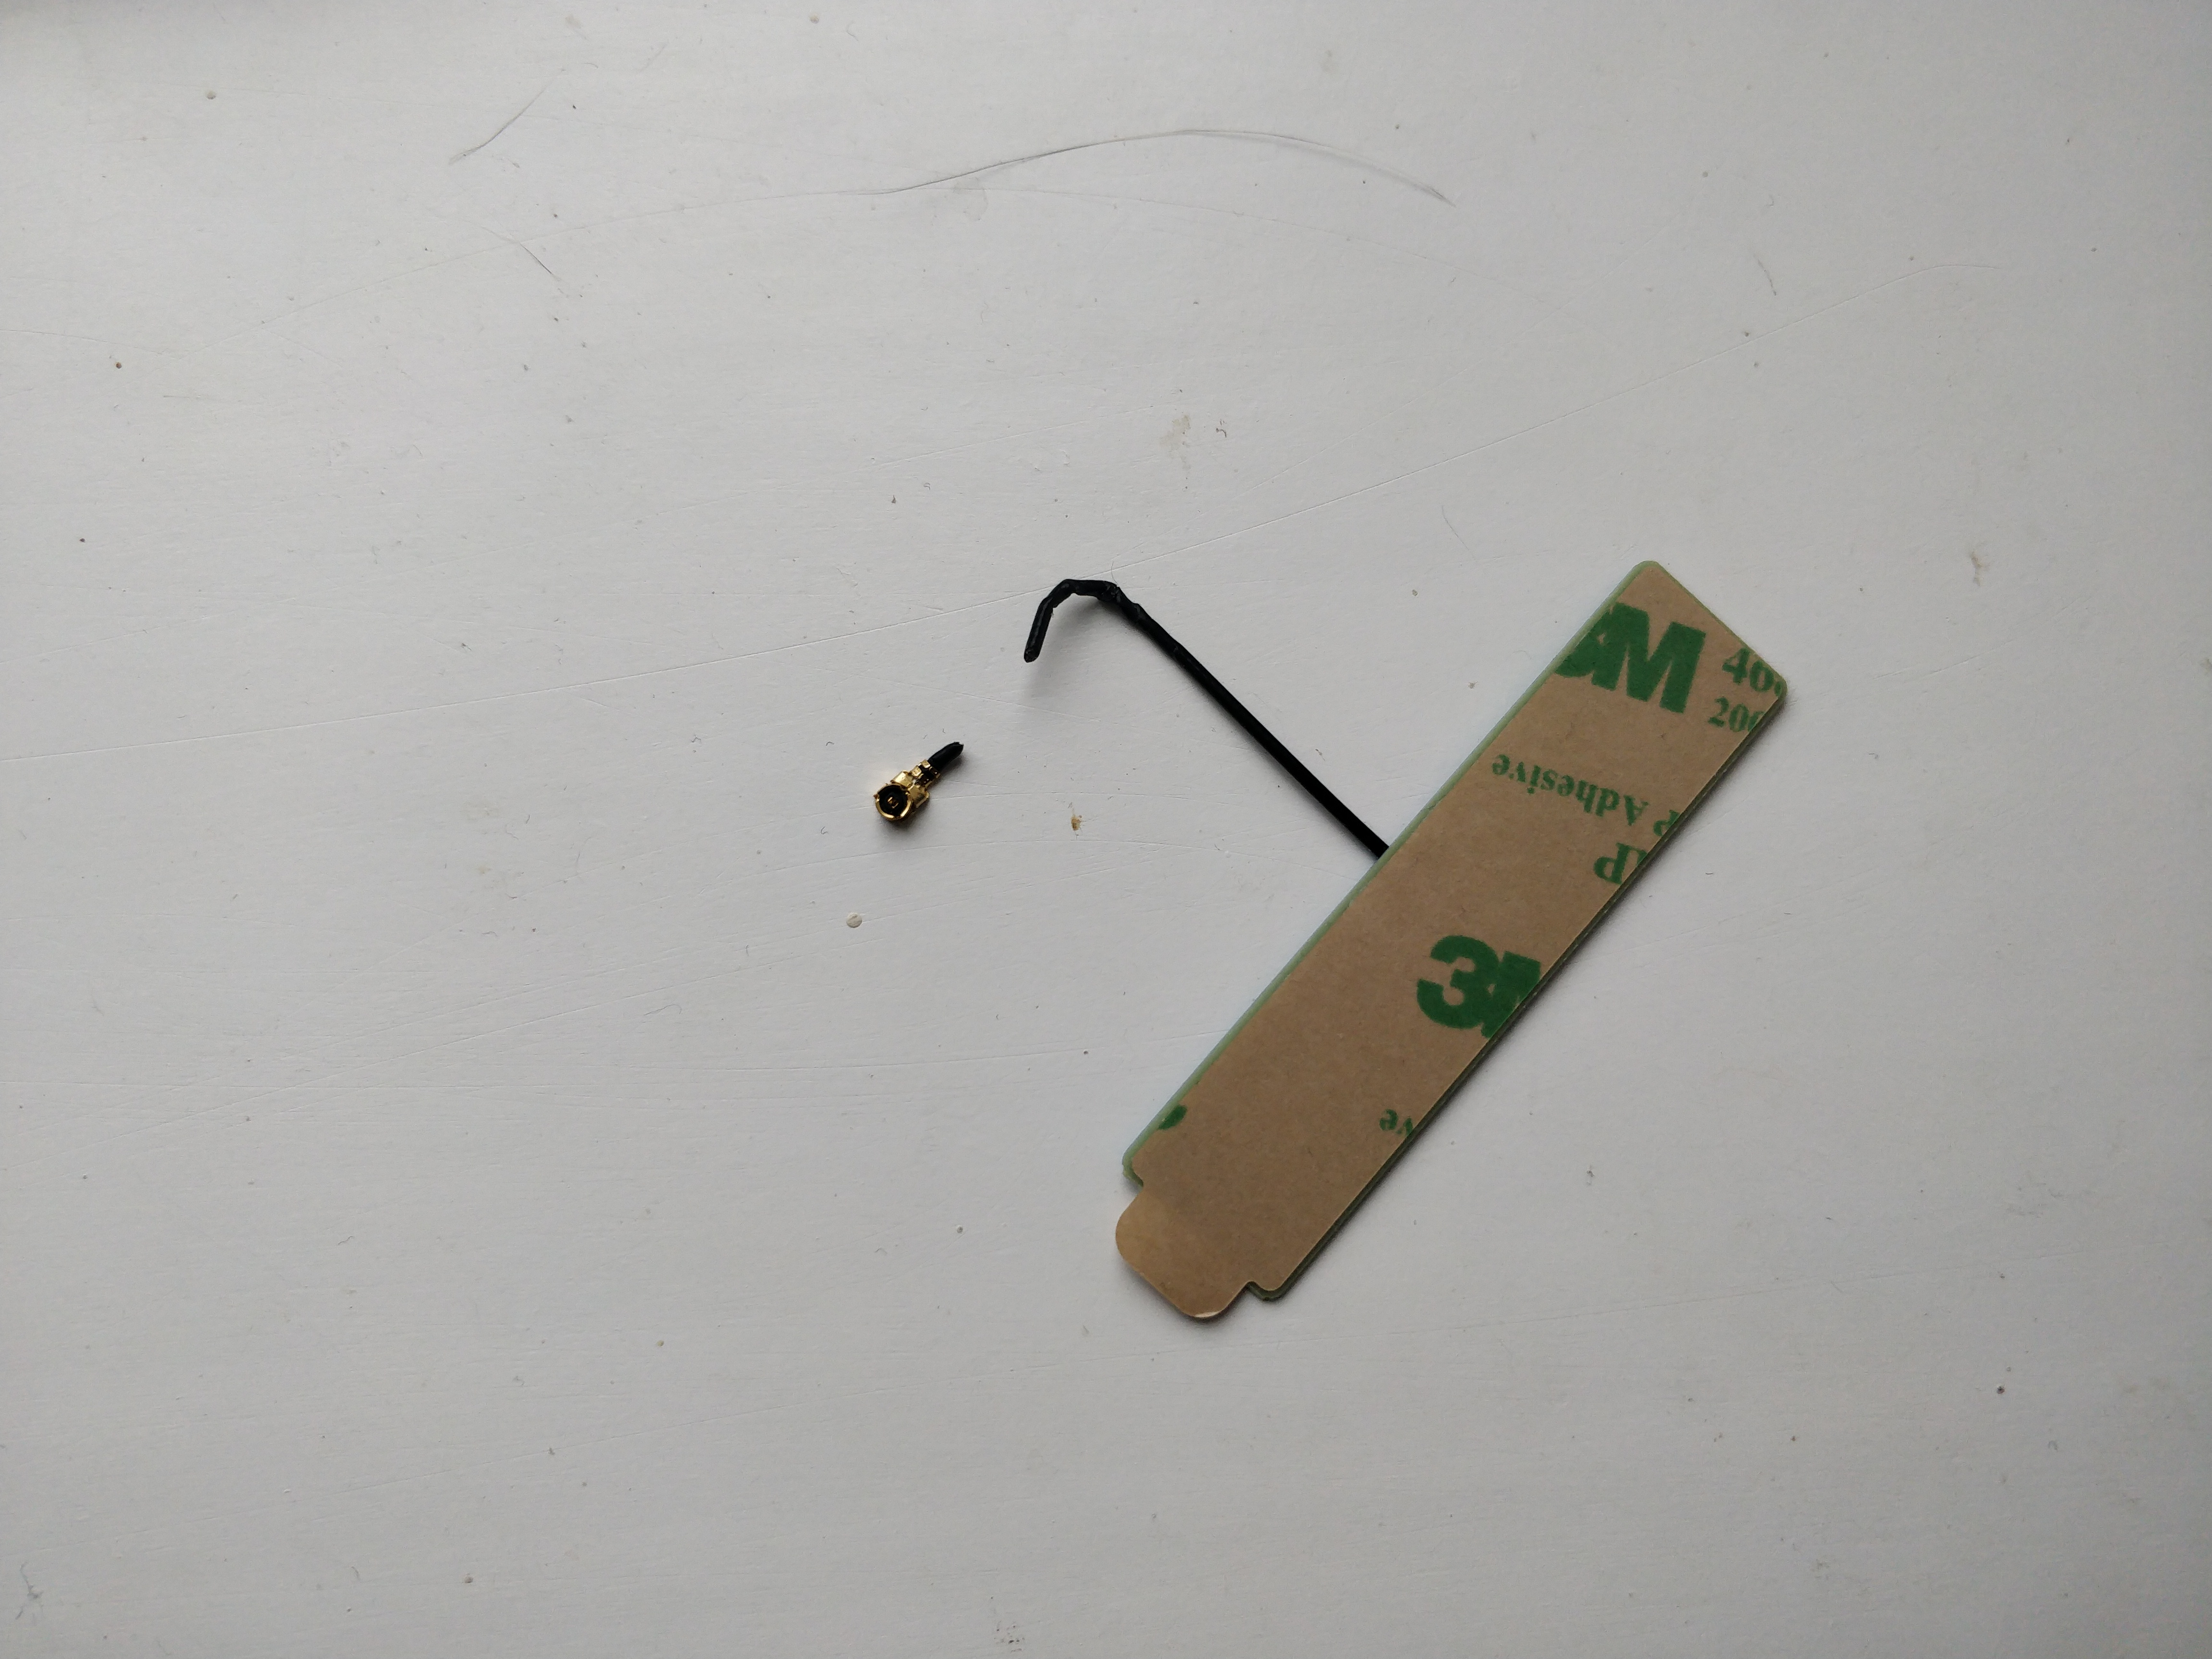
\includegraphics[width=0.4\textwidth]{../figures/damaged antenna.jpg}
    \caption{Damaged strip antenna.}
    \label{fig:damagedantenna}
\end{wrapfigure}

Due to delivery issues, neither module currently is able to use an antenna, and thus have
been confined to short range tests only.
While part of the purchasing list included ceramic and strip antennae for the
transmitter only, the ceramic antennae cannot be used as they require some form of breakout,
usually on a \acrshort{pcb} and further currently require a \gls{ufl} adapter to interface
with the board. The strip antenna, on the other hand, use a very delicate cable between the strip itself and
the connector, and were therefore easily sheared by one \textit{Felis catus} who found it
unattended during operation.

% \begin{figure}[H]
%     \centering
%     % \captionsetup{justification=centering}
%     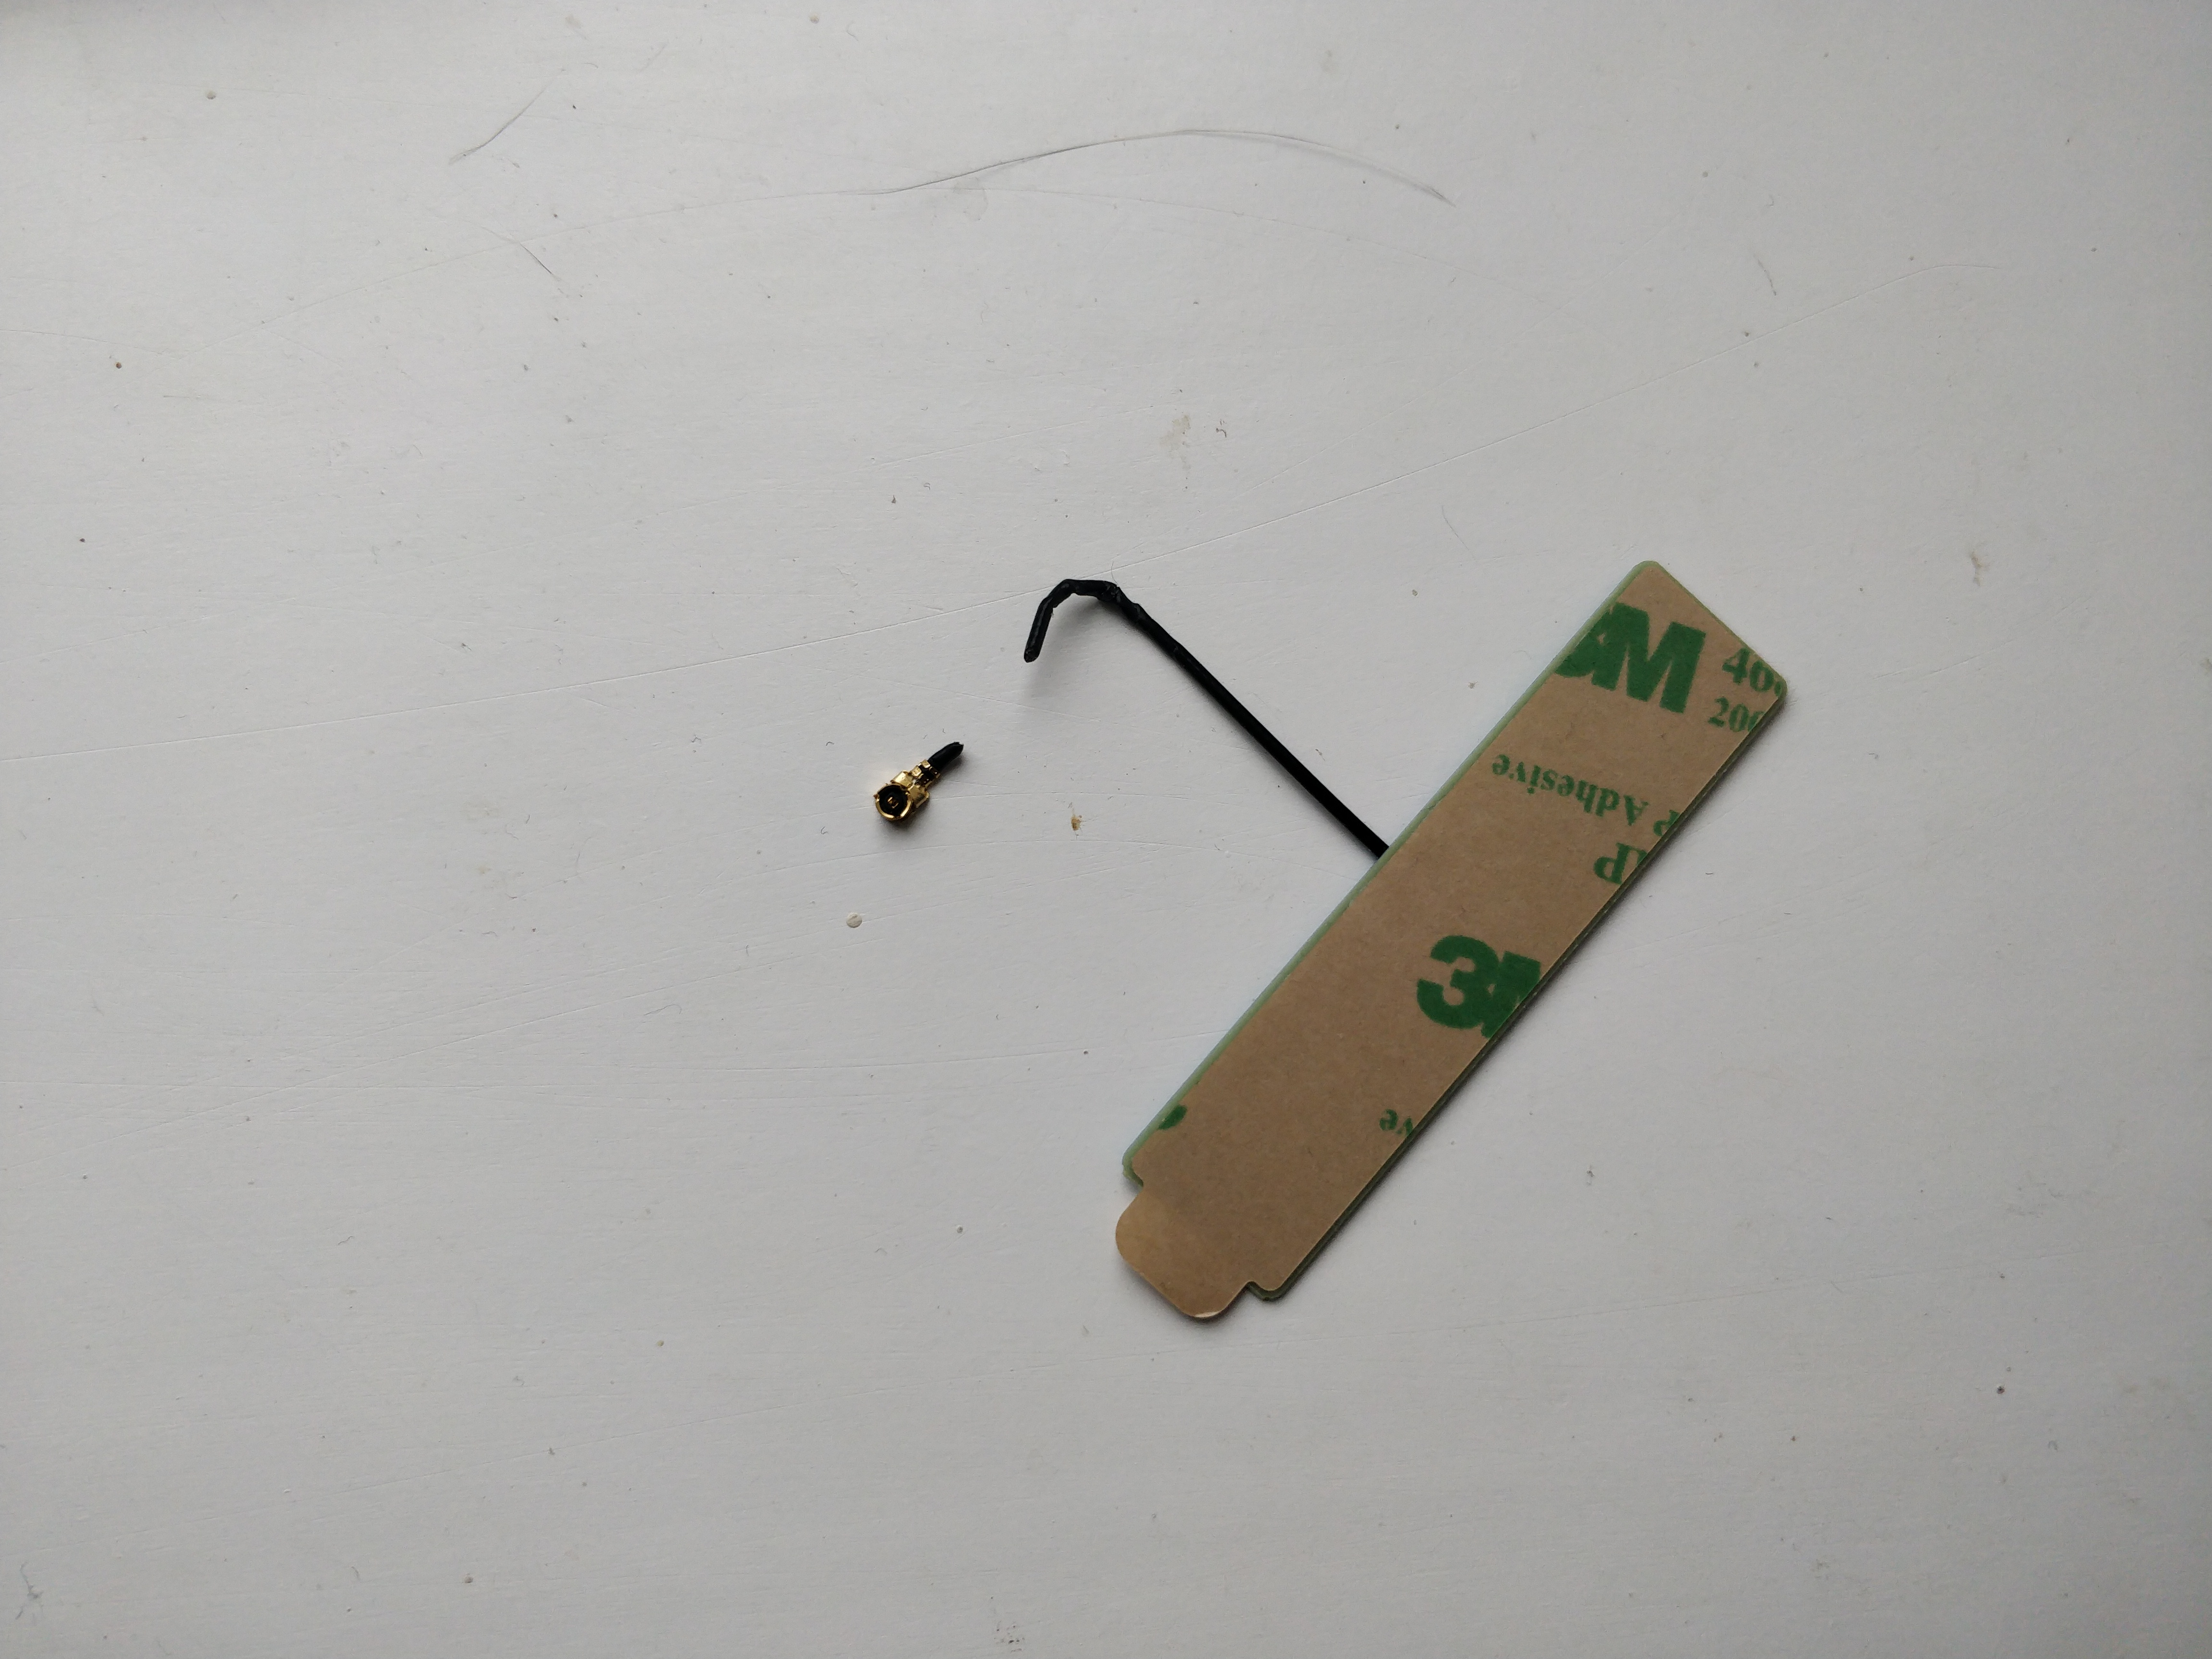
\includegraphics[width=0.4\textwidth]{../figures/damaged antenna.jpg}
%     \caption{Damaged strip antenna.}
%     \label{fig:damagedantenna}
% \end{figure}

A spare whip antenna was available to use with the Pi, however its frequency was
unknown. Upon casual inspection, it may be appropriately sized. To investigate further,
the appropriate antenna length needs to be determined.

The wavelength can be found by:
\begin{align*}
    \lambda & = \frac{v}{f}
\end{align*}

\begin{conditions}
    \lambda & = & wavelength \\
    v & = & velocity, which in this case will be $c$, the speed of light \\
    f & = & frequency \\
\end{conditions}

% where: 

% \begin{tabular}[H]{ l c l}
%     $\lambda$ & $=$ & wavelength \\
%     $v$ & $=$ & velocity, which in this case will be $c$, the speed of light \\
%     $f$ & $=$ & frequency \\
% \end{tabular}\\

For the device operating at \qty{868.0}{\MHz}, this appears like the following:
\begin{align*}
    \lambda & = \frac{c}{\qty{868.0}{\MHz}} \\
            & = \qty{0.345}{\m}
\end{align*}

The antenna whip measures between \qty{21}{\cm} and \qty{25}{\cm}, although
it is impossible to say exactly how long it is without opening it up.
If this antenna is centred near \qty{868}{\MHz}, it may be a five-eighth whip, given
$\frac{5}{8}\lambda = \qty{21.5}{\cm}$. This suggests it is appropriate to use until 
a more robust set of antennae has requested for ordering\footnote{
    Decided list can be found in \cref{table:antennaelist}.
}.

\subsection{Battery test}

The purpose of the test is to determine the length of time the transmitter can continuously
operate under normal conditions, i.e. obtaining current \acrshort{gps} location and
transmitting it via \gls{lora}.
As outlined in \cref{sec:powertestspec}, there is an expectation of roughly eight
hours of function. This will now be investigated to determine whether this is the case.

The transmitter code will need to be updated to include information about the current
status of the battery. The voltage level of the battery indicates whether it is
within operating range, which can be measured by reading the analogue value of
pin \lstinline{A7}. At \qty{4.2}{\V}, capacity as it maximum, whereas the board
will cease function around \qty{3.2}{\V}. The exact calculation can be found in
the board documentation \cite{adafruit:loram0}, which has been adapted in \cref{arduino:bat}.

After ascertaining that the calculation was working correctly, the code has been included in
\cref{arduino:lpgps2}\footnote{
    This is in fact the third iteration of code. The two former versions can be found in \cref{arduino:serialgps} and \cref{arduino:libgps}.
}. The output string has also been modified to include the battery data,
altitude, and fix quality.
\acrshort{gps} fix takes the following values \cite{arcgis:gpsfix}:

\begin{description}[align=left, labelwidth=1cm,labelindent=0.5cm]
    \item[0] No fix (no signal)
    \item[1] Position fixed with \acrshort{gnss} satellites
    \item[2] Differential \acrshort{gps}
    \item[3-5] \acrshort{pps}\footnote{Encrypted military/government use}/\acrshort{rtk} fix
    \item[6] Estimated location
        \label{table:fix}
\end{description}

The latter two
required \gls{gpgga} data, which can be included with the library command
\lstinline{PMTK_SET_NMEA_OUTPUT_RMCGGA}. Finally, field separators were replaced with commas
as part of preparation for the data to be stored in \acrshort{csv} format.

\subsubsection{Test parameters}
Two tests were conducted.
\begin{enumerate}
    \item Discharge - The board operates under normal conditions. The battery was
          charged to maximum capacity (\qty{4.2}{\V}), before being allowed to discharge
          completely. Throughout that time, the board was transmitting
          location data and battery level. The receiver logs the time of
          packets and stores it in a data structure.
    \item Charge - After a complete discharge, the time taken to charge to maximum
          was recorded similarly.
\end{enumerate}

The way the Pi is operated was changed. Normally, an \acrshort{ssh} session
is terminated when the client disconnect or times out, and any programs run during that
session are closed. This was not a problem with the
power meter test as the receiver only needed to indicate that transmitter was working,
while the data itself was recorded externally. In this case, the Pi is recording all data
and needs to be running without interruption for at least eight hours.
Linux comes with a utility named
\lstinline{screen} that allows a virtual terminal session to be started that will
not be closed\footnote{An alternative
    would be to run the process and move it to background. The benefit of \lstinline{screen} is that
    logging messages are easier to view when printed to terminal.}.

\paragraph{Risks}
The greatest risk is related to the battery short-circuiting, however this 
has been dealt with adequately in \cref{sec:intermediate}. 
It is possible the battery may be damaged due to excessive discharge,
however the protection circuitry will cut the supply before then. 

\subsubsection{Issues}
The tests were executed without issue and a brief study of the results indicated they
were within expectation. However, some issues cropped up.

C treats strings as an array of type \lstinline{char} and determines
the end of the string with the `null' character\footnote{In two byte
    hexadecimal representation as an escape character, \lstinline{\\x00}.} `\lstinline{\0}'.
C++ carries this over. Thereby, when using the C++ \lstinline{String} class,
this behaviour remains. As it is treated as part of the string, it is furthermore
included in the length calculation and therefore transmitted over \gls{lora}.
The receiver would then interpret the characters of the packet in \lstinline{utf-8},
and translate the null character as \lstinline{\x00}. The existence of null characters
introduces difficulty when attempting to interpret the file in \acrshort{csv} format.

The eventual solution was to perform packet processing on receipt, 
as cleaning the files manually had thus far failed.
The inbuilt \lstinline{rstrip()} method on a string type allows a specific character
(in this case, \lstinline{\x00}) to be removed. 

Additionally, supplementary information, like errors, were logged to console
with extra diagnostic information instead of stored in the file.
Beforehand, this information would have to be stripped as the error line was non-standard for
the \acrshort{csv} format\footnote{
    The producing code can be found in \cref{pi:first}.
}. An example is shown in \cref{table:errorlogex}.

{\small
\begin{xltabular}{\linewidth}{|ccllll|}
    \hline
    \rowcolor{tableh1}
    Date & Time & Packet & Longitude & Latitude & Voltage \\
    \hline
    23/01/27    & 20:27:27  & 3040  & 0	    & 0  & 4.15  \\
    23/01/27	& 20:27:32	& 3041	& 0     & 0  & 4.15  \\
    23/01/27	& 20:27:35	& unicode parse error & & &  \\
    23/01/27	& 20:27:32	& 3041  & 0     & 0  & 4.15  \\
    23/01/27	& 20:27:37  & 3042	& 0	    & 0  & 4.157 \\
    23/01/27	& 20:27:42	& 3043	& 0	    & 0  & 4.15  \\
    \hline
    \caption{Non-standard format example - 230127.csv sample}\label{table:errorlogex}
\end{xltabular}
}

This would cause errors for the \acrshort{csv} interpreter due to mismatched
field lengths.

Finally, plotting temporal data types proved to be problematic.
To simplify this, two changes were made: firstly, the Date and Time fields
were collated into one field in the standard format MATLAB expects\footnote{
    Format: 1\textsuperscript{st} February 2023 at 1:54pm as ``01-02-23 13:54:00''.
}; secondly, a field was added for recording time relative to Unix epoch
(i.e. now completely numeric and linear) in case plotting with such a field
proves simpler.

The tests were then performed a second time.

\subsubsection{Results}
Data samples of the results can be found in \cref{table:dischargedata} and \cref{table:chargedata}.
The resulting plot is shown in \cref{fig:batteryplot} using code in \cref{script:batteryscript2}\footnote{
    This is the second version of plotting code. The first can be found in \cref{script:batteryscript1}.
}.

\begin{figure}[H]
    \centering
    \includegraphics[width=\textwidth]{../../Code/Tests/Battery/Figure_4.png}
    \caption{Battery charge and discharge curves}
    \label{fig:batteryplot}
\end{figure}

The plots show the battery voltage level and whether the \acrshort{gps} has a fix.

\paragraph{Discharge}
Recording starts with a full battery, indicated by \qty{4.2}{\V}. Operation
continues as expected, with \acrshort{gps} location fixed for much of that time.
On two occasions, the fix was recorded at a value of 6\footnote{
    Reference in \cref{table:fix}.
}.
\acrshort{gps} was not unavailable for long enough to indicate whether not having a fix
has any significant impact on battery consumption.
Overall, the data indicates the total useable span of the device is fifteen hours.

\paragraph{Charge}
Notably, the voltage at the point of charging is much lower than was last recorded
when transmission during discharge cut off. The board does in fact continue to draw power.
This ceases when the protection circuitry of the battery cuts supply entirely. This leads to
some parasitic draw in the elapsed time. \acrshort{gps} location fix did not have a
noticeable effect upon charging. Total time to charge to full capacity was around
five hours and thirty minutes.

\paragraph{Remarks}
The discharge results were surprising. The estimate calculation
\cref{sec:powertestspec} returned an expectation of eight hours of function.
Despite being a conservative estimate, the experimentally found value was
almost double this. Furthermore, additional power saving functions like
putting the radio to sleep when not in use were not used, meaning the operating
time of the device can be further increased\footnote{
    Transmission was set at \qty{5}{\s}, which is better than specified in \cref{sec:timing}.
}. 

The time required to charge the module to maximum capacity was
greater than expected. The slow charging time may come down to
a few reasons. The charging regulator built into
the Feather board is current limited to protect the circuitry \cite{adafruit:loram0}.
It is further limited by the maximum current a \acrshort{usb} 2.0 connector can draw
(\qty{100}{\mA}) \cite{axelson:usb}. This can be negotiated to be greater \cite{ftdi:usb}, however,
and certainly many modern devices, particularly mobile phones, utilise some form of rapid charging.

The data collected suggests reliability. Any moment-to-moment fluctuations will be smoothed out
due to the operating time of the module, so further tests
may not be necessary. Furthermore, it is not advisable to repeatedly charge
and discharge lithium cells from maximum to minimum as doing so reduces the lifespan of the cell.

\subsection{Error investigation}
Further insight may be gained on the corrupted packets\footnote{\Cref{sec:codeissues}.}.
The errors recorded before the discharge test was performed can be found in \cref{error:decoding}.
It is notable that there are fewer errors here than in previous tests. The only significant change
was the use of antennae during transmission. To elaborate on the error message, many of the bytes
in the byte array cannot be decoded as they are all invalid \lstinline{utf-8}, not just the start byte.
The structure should follow 8-bits per character, yet some are greater (\lstinline{\x90w}, line 13), use invalid
hexadecimal (\lstinline{\xb8B}, line 13), or are entirely not present (\lstinline{\x89\\22Rs}, line 4).
\begin{itemize}
    \item Invalid hexadecimal - This appears due to the way Python \lstinline{bytearray} is used. Where the
          default decoding (\lstinline{utf-8}) failed, the array
          is encoded as \lstinline{ASCII} and printed to console.
          This leads to non-hexadecimal characters appearing, and likely some of the missing characters also.
    \item Not 8-bits - If, for example, during transmission part of a byte is lost,
          the remainder of the packet will
          fail to decode correctly and appear in different lengths and otherwise non-standard form.
\end{itemize}

\paragraph{Solution}
There is no simple solution to what is essentially the question of how to ensure data integrity
during transmission in a noisy environment. The RadioHead library supports packet confirmations
with the \lstinline{RHReliableDatagram} class. This does not validate the packet
integrity\footnote{A single bit being flipped may still resolve to a valid packet,
    even if the data is no longer accurate.}, but ensures that the packet has arrived. This
solution alone would require some reverse engineering of the \lstinline{recvfromAck} method
in order to use it on the receiver end, however can be used to request retransmission (i.e.
fail to acknowledge the packet) should it arrive corrupted.

An alternative would be to utilise some form of forward error correction, like parity checking.
This has the limitation of increased complexity and computational load on the transmitter,
and is further limited by being able to correct only one error. To adequately cover the
entire transmission, the packet size (and subsequently, radio power draw and processor time)
would increase.

The corrupted packets are few and infrequent enough (only one at a time) that 
they can simply be omitted. As reporting is set to \qty{5}{\s}, up to five 
packets can fail in a row for the specification of \qty{30}{\s} reporting to be met. 
Moving the device to production would require a revisit of handling data integrity.


\subsection{Case design}

In preparation for the distance test, ensuring the electronics were, at minimum,
protected from damage increased in importance. 
The case will be attached to a cat harness or collar as a complete unit (i.e. sewn in),
however this level of integration will be paused until the hardware is moved onto a \acrshort{pcb}
with smaller form-factor. Instead, the purpose of this case design will be to 
provide a protective enclosure for the period of function testing the tracker. 

\begin{wrapfigure}[9]{R}{0.3\textwidth}
    \vspace{-5pt}
    \centering
    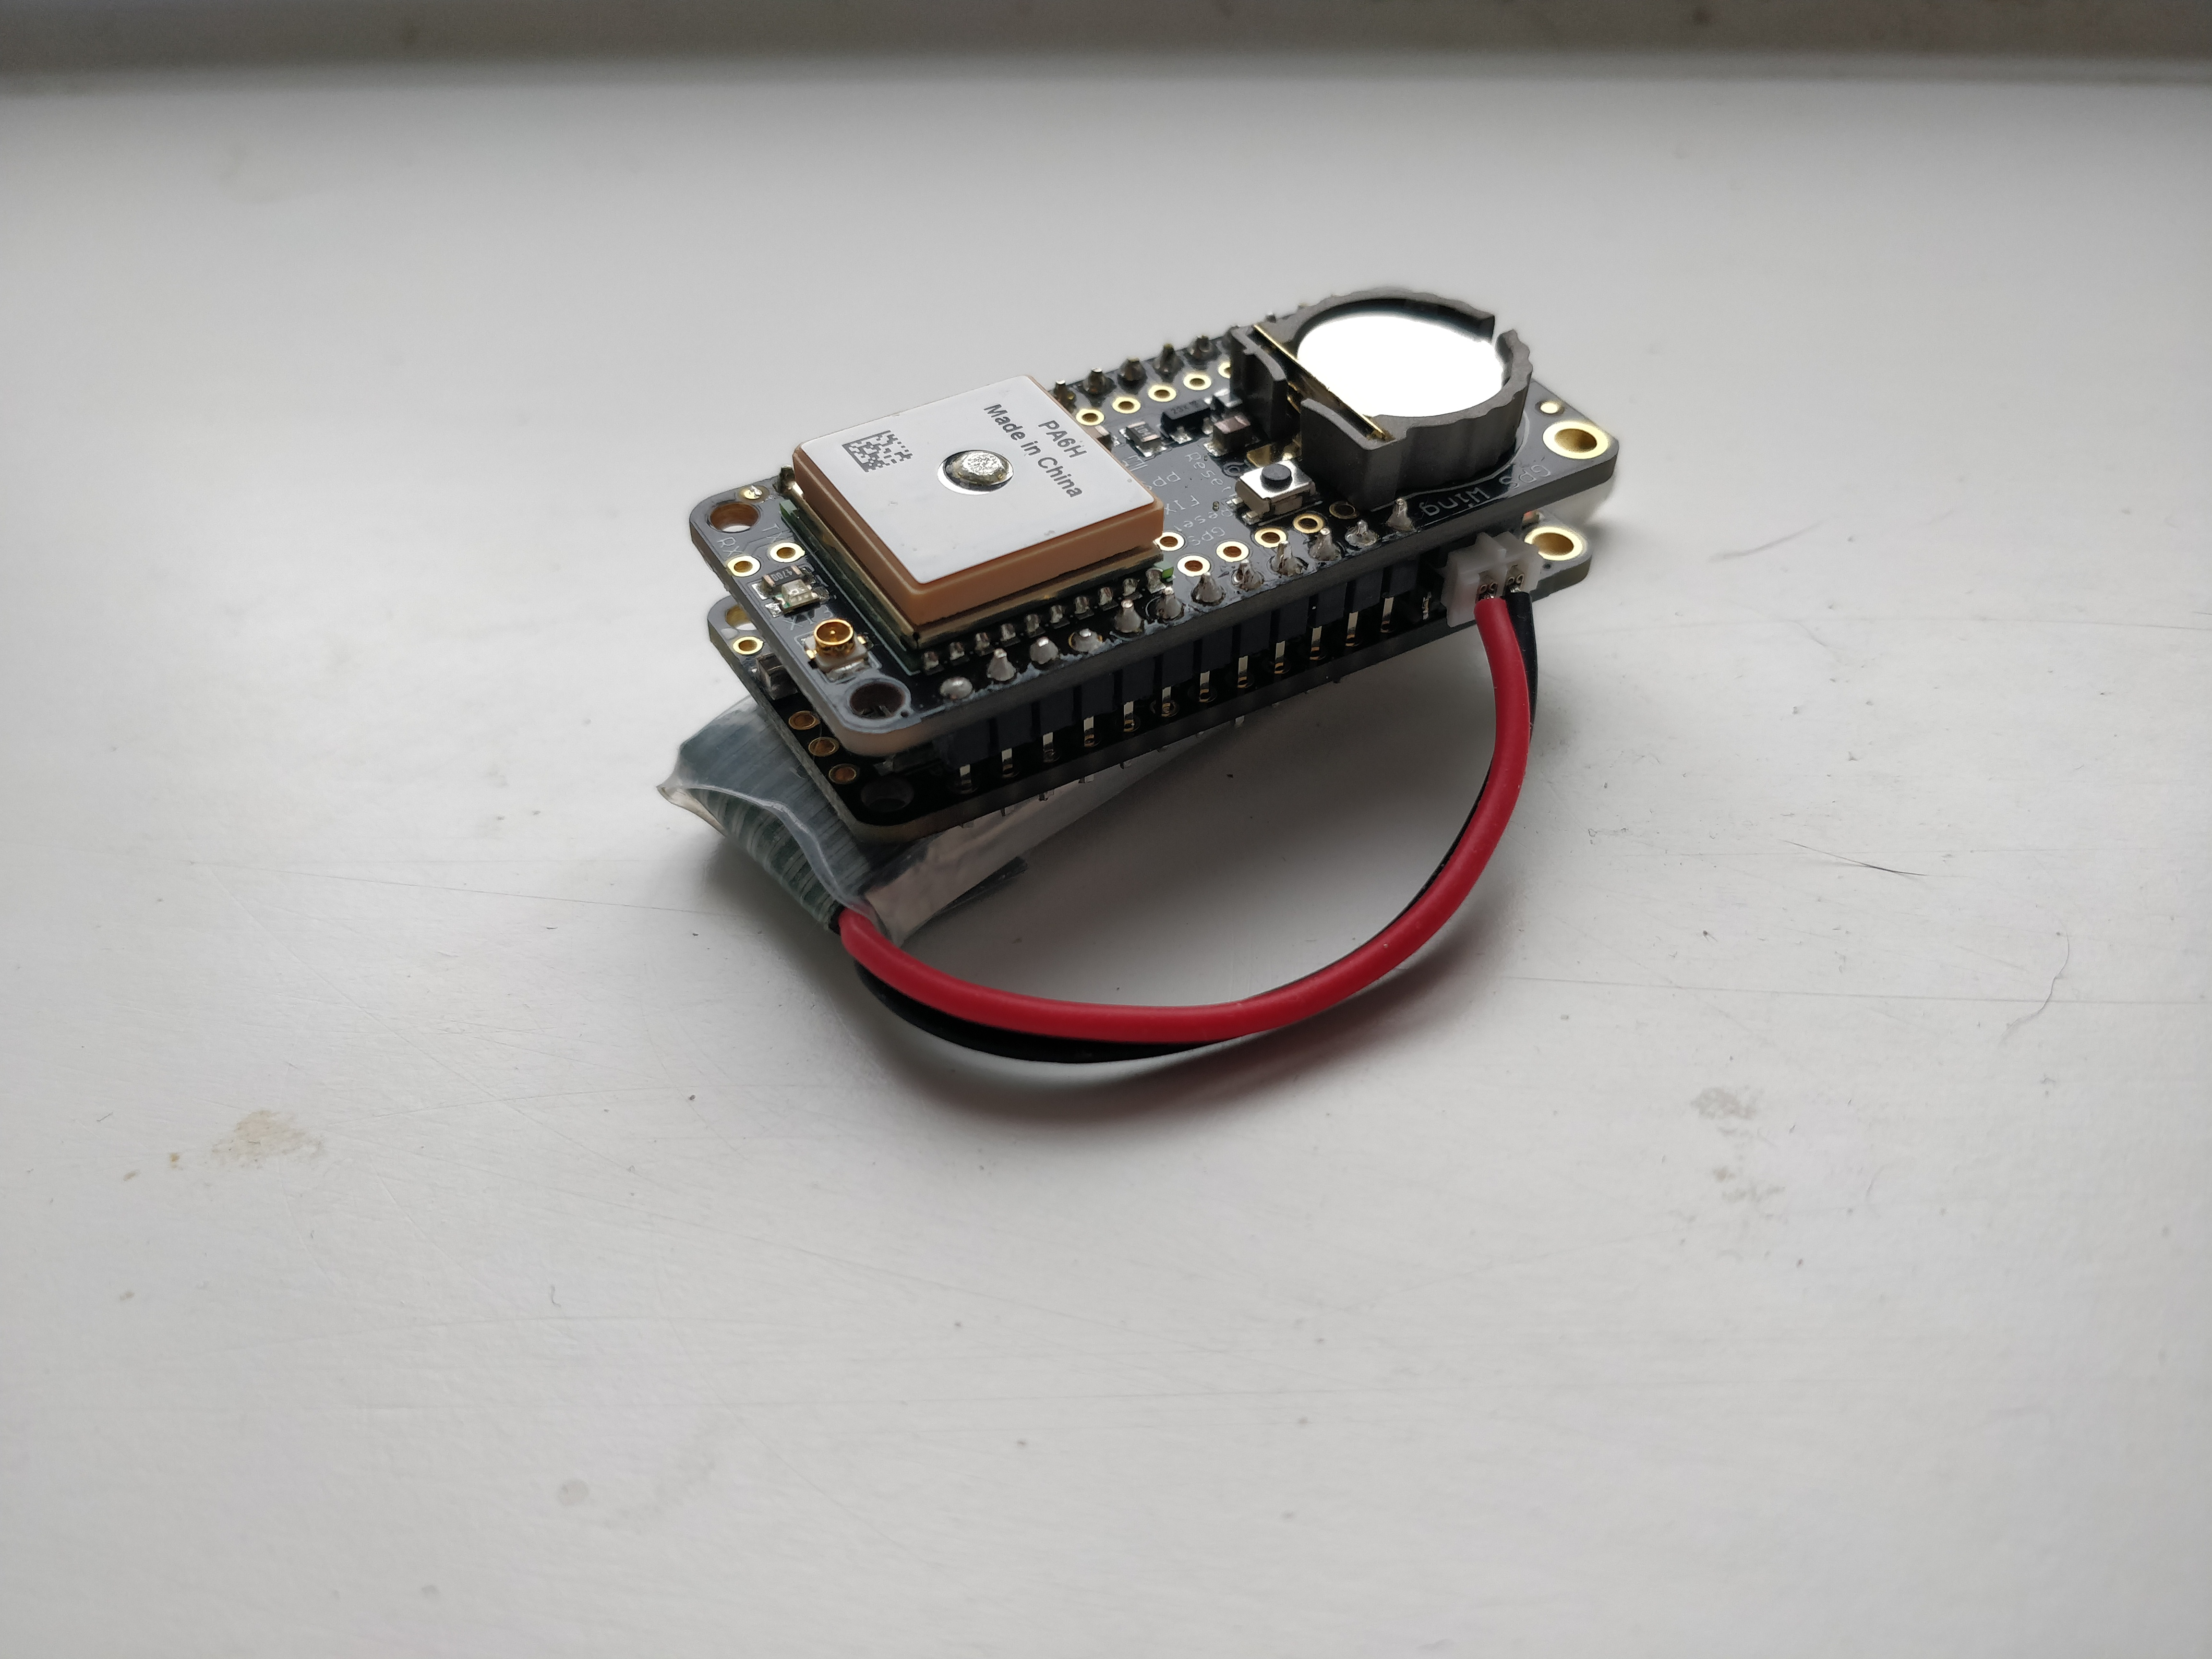
\includegraphics[width=0.3\textwidth]{../figures/Pics/bareboard.jpg}
    \caption{Board and battery at the beginning of case development}
    \label{fig:bareboard}    
\end{wrapfigure}

% \begin{figure}[H]
%     \centering
%     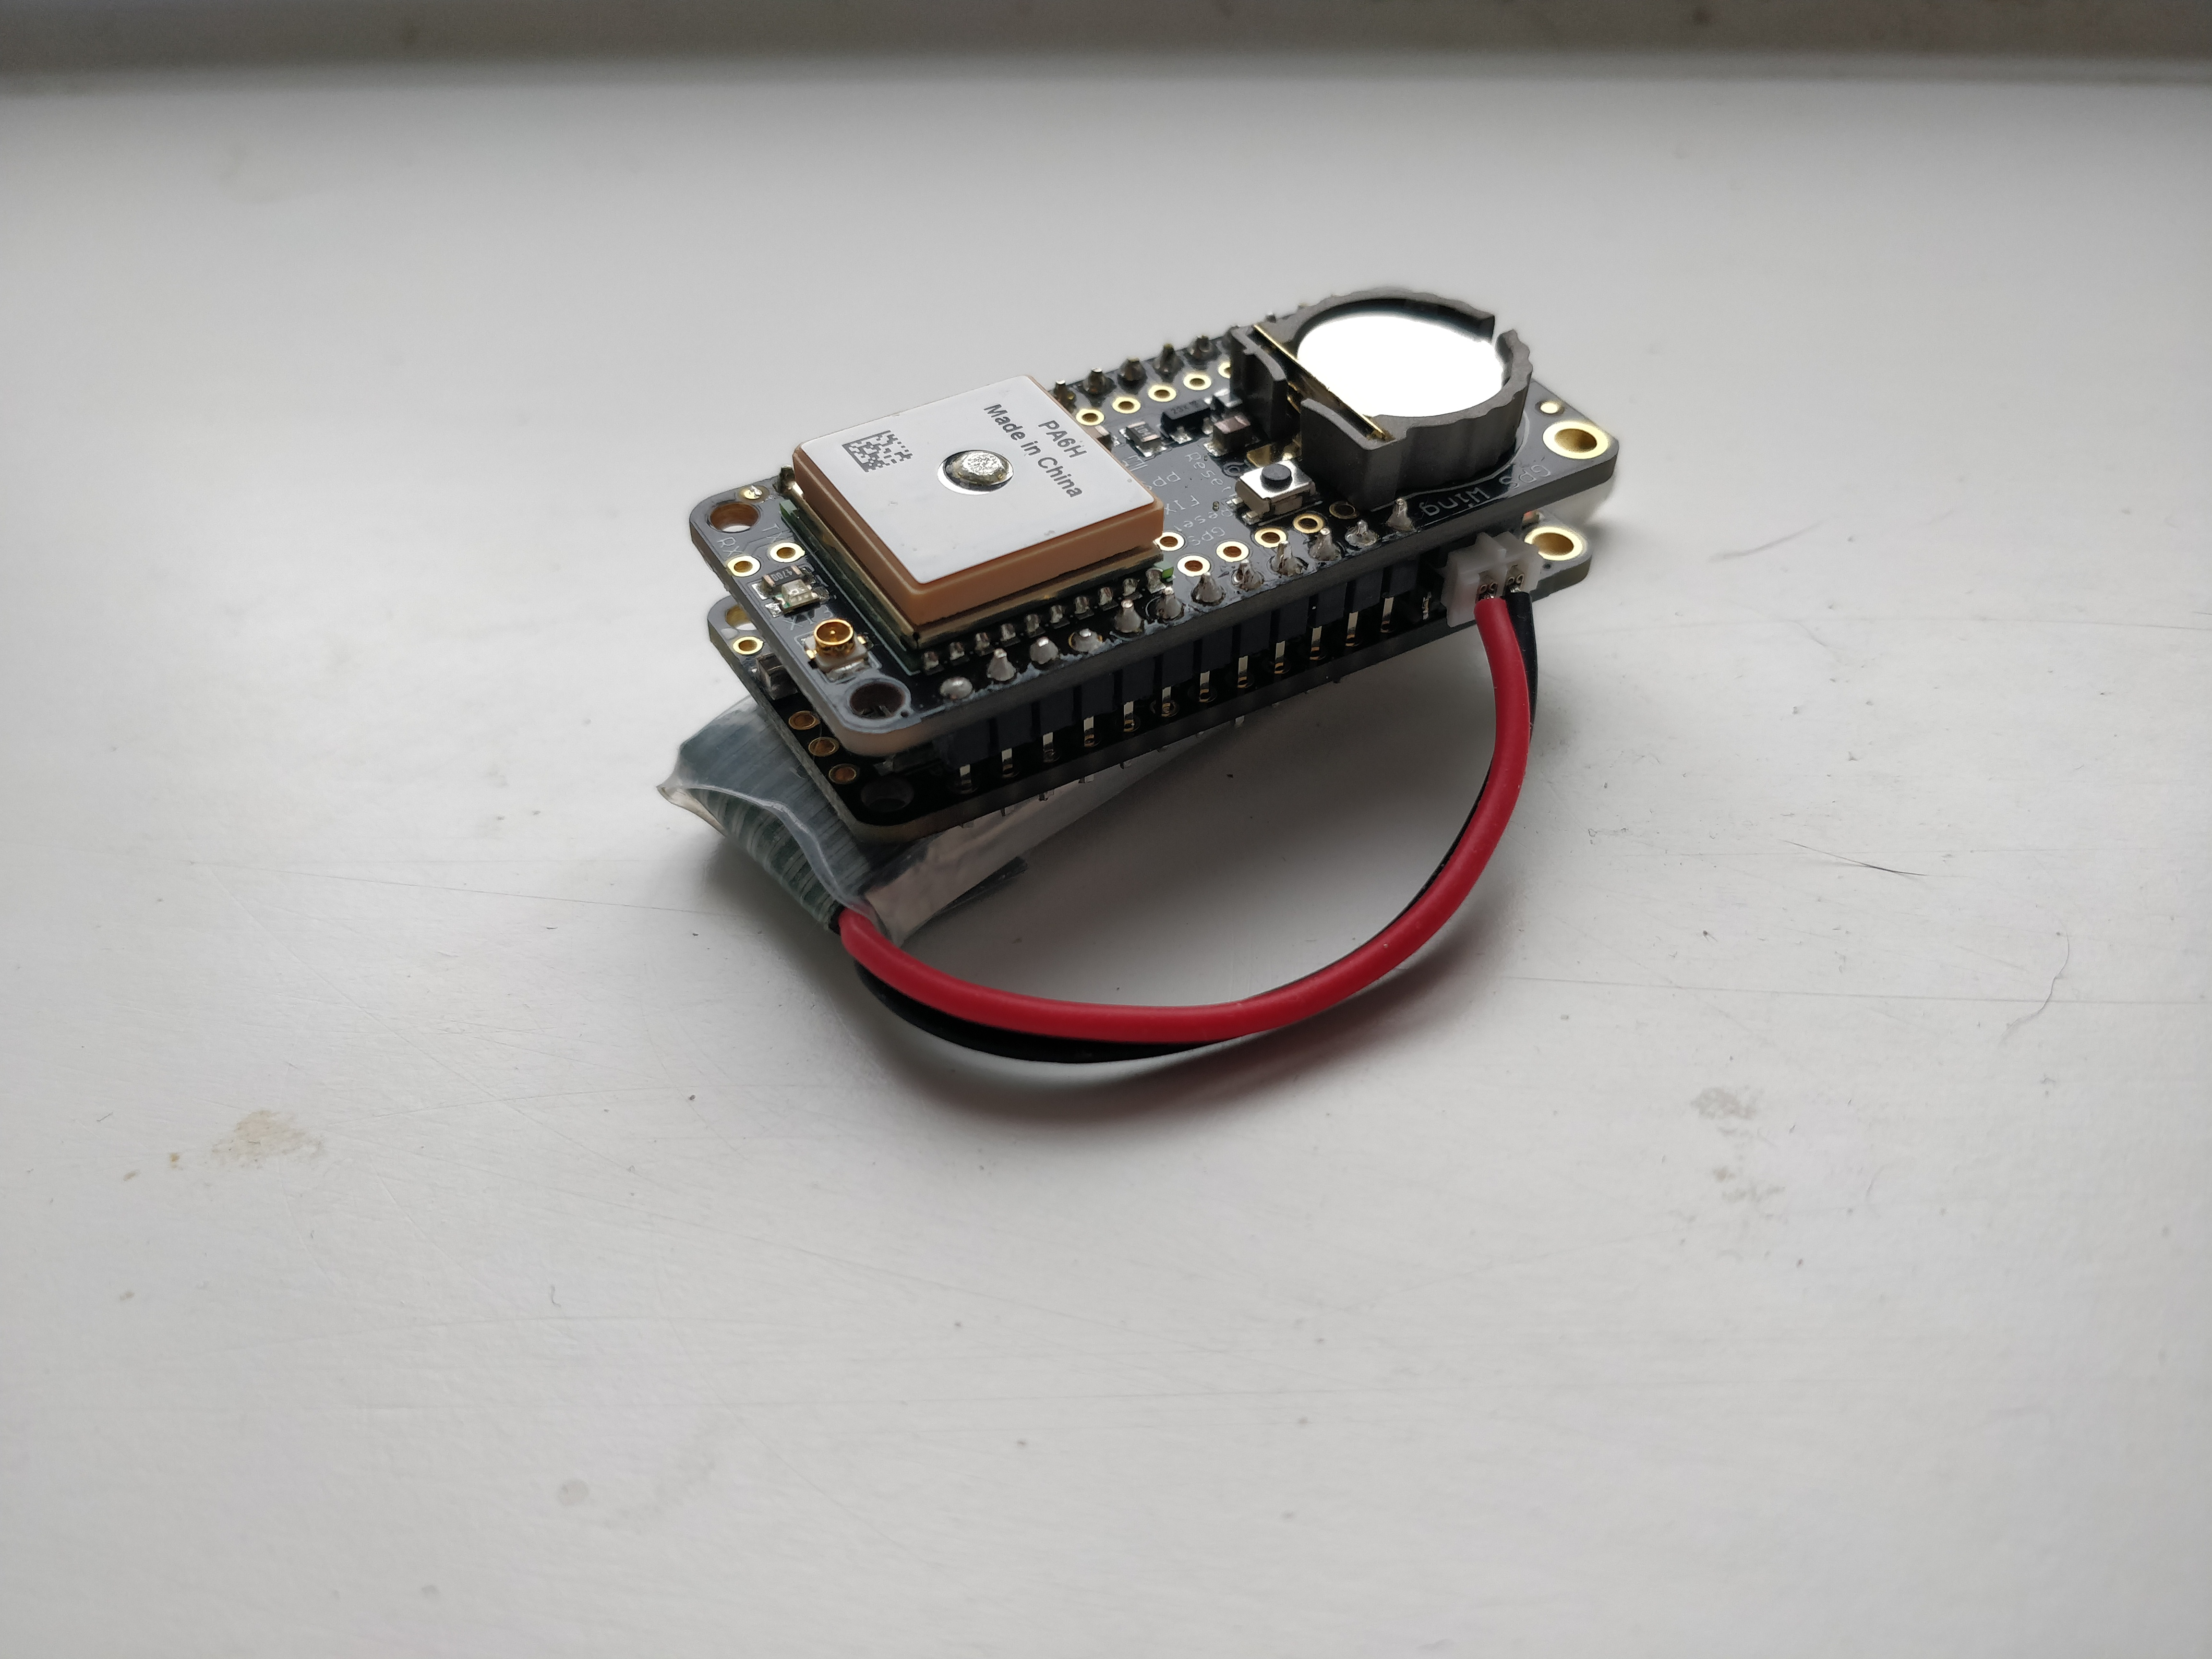
\includegraphics[width=0.7\textwidth]{../figures/Pics/bareboard.jpg}
%     \caption{Board and battery at the beginning of case development}
%     \label{fig:bareboard}
% \end{figure}

\Cref{fig:bareboard} shows the board when development of the case started (especially
showing the stacked height).
As can be seen, the connecting wires between the battery and board were a potential
point of failure. Furthermore, in the process of disengaging the battery repeatedly
to remove power and halt battery drain (due to no current off-switch available),
the wire sheath had pulled back to expose the stranded core\footnote{This became
    bad enough that a makeshift cover made from insulting tape was added to ensure the wires
    did not short circuit - as can be seen most clearly in \cref{fig:case1top}.
}.

% \vspace{33pt}
Two key factors drove considerations for the case development:
\begin{itemize}
    \item Due to mismatched sizing between the battery and board, both had to be enclosed, so they
          would not rock about in the casing.
    \item Given the stage in development and likelihood of frequent easy access, the components
          were separated to best allow easy access, even at the expense of the smallest volume possible.
\end{itemize}

\subsubsection{First case}
\paragraph{Design}
The case was modelled in Autodesk Fusion 360 after measurements were taken
of the components. A raised battery platform with rounded
edges was created to hold the battery. The board takes up noticeably less space and
therefore a cage was modelled to house it securely. An arch was included to allow the
battery connection port to remain available. The lid was designed to fit in the casing
recess. Due to the tendency for \gls{fdm} parts to widen when laid, a fillet was
included in the lid lip to allow room for this. Extra space for the power cabled to
come out of the front of the battery was provided.
Finally, holes were added on all vertical
sides to allow an antenna to be routed through wherever most convenient.

Dimensional drawings for the case can be found in \cref{fig:case1dwg}.

\paragraph{Manufacture}
\label{sec:case1manufacture}
The manufacturing method of choice was 3D printing using an Ultimaker 3 \gls{fdm} printer.
In order to print the casing, it would first have to be `sliced' and encoded into \gls{gcode}.
The software chosen to do this was Ultimaker Cura, as it supported Ultimaker printers natively.
Default `fast' settings were used as the casing was a prototype and therefore dimensional
precision is of less importance. Due to large overhangs in the board enclosure, especially at
the battery port, the head movement speed was increased by 15\% in order to bridge the gaps.
Doing so increases the risk of small features like the pillars to fail due to insufficient time
for the layer to cool. The increased bridging capability meant that supports could be disabled,
however the gap for the battery port would have been too large to bridge without supports,
and was therefore modified into an arch to support itself.

\paragraph{Result}
The first print failed due to an extruder blockage towards the end of the first layer
being completed. As this occurred after the period of observation to ensure successful
printing, the issue was only apparent the next day. The result can be seen in \cref{fig:failedprint}.

% \begin{figure}[H]
%     \centering
%     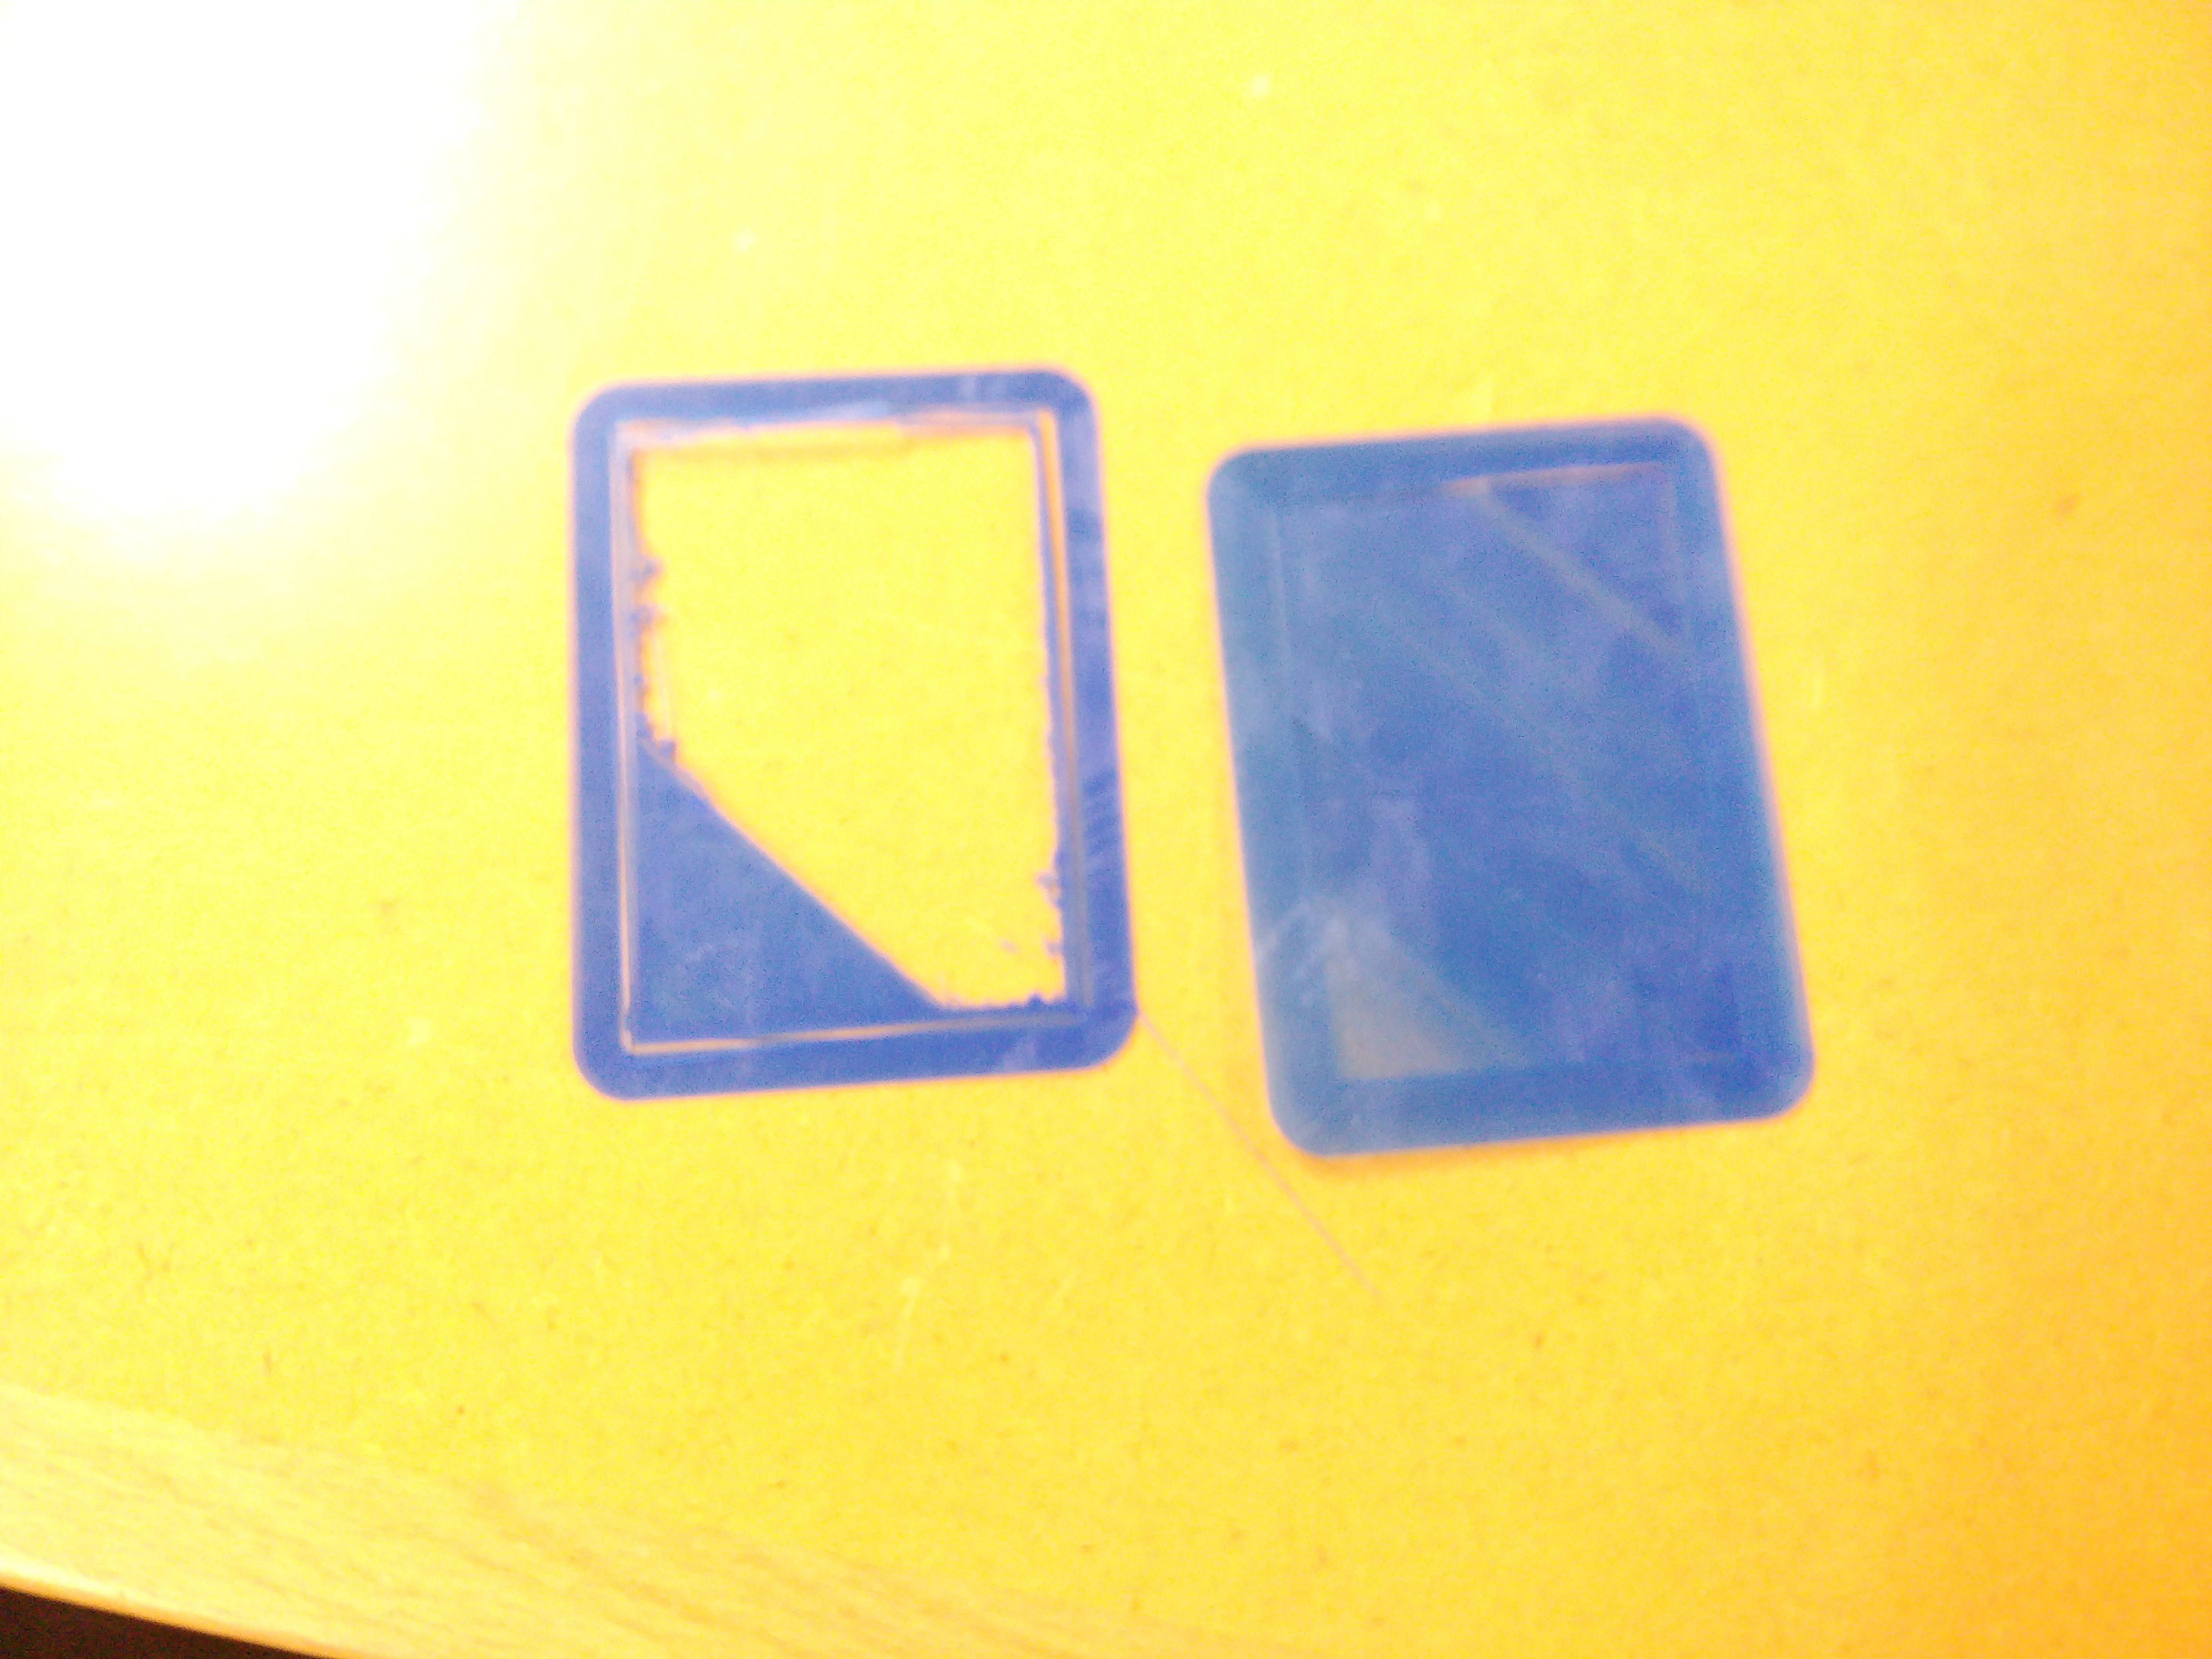
\includegraphics[width=0.7\textwidth]{../figures/Pics/failedprint.jpg}
%     \caption{Failed print}
%     \label{fig:failedprint}
% \end{figure}

\begin{wrapfigure}{L}{0.3\textwidth}
    \centering
    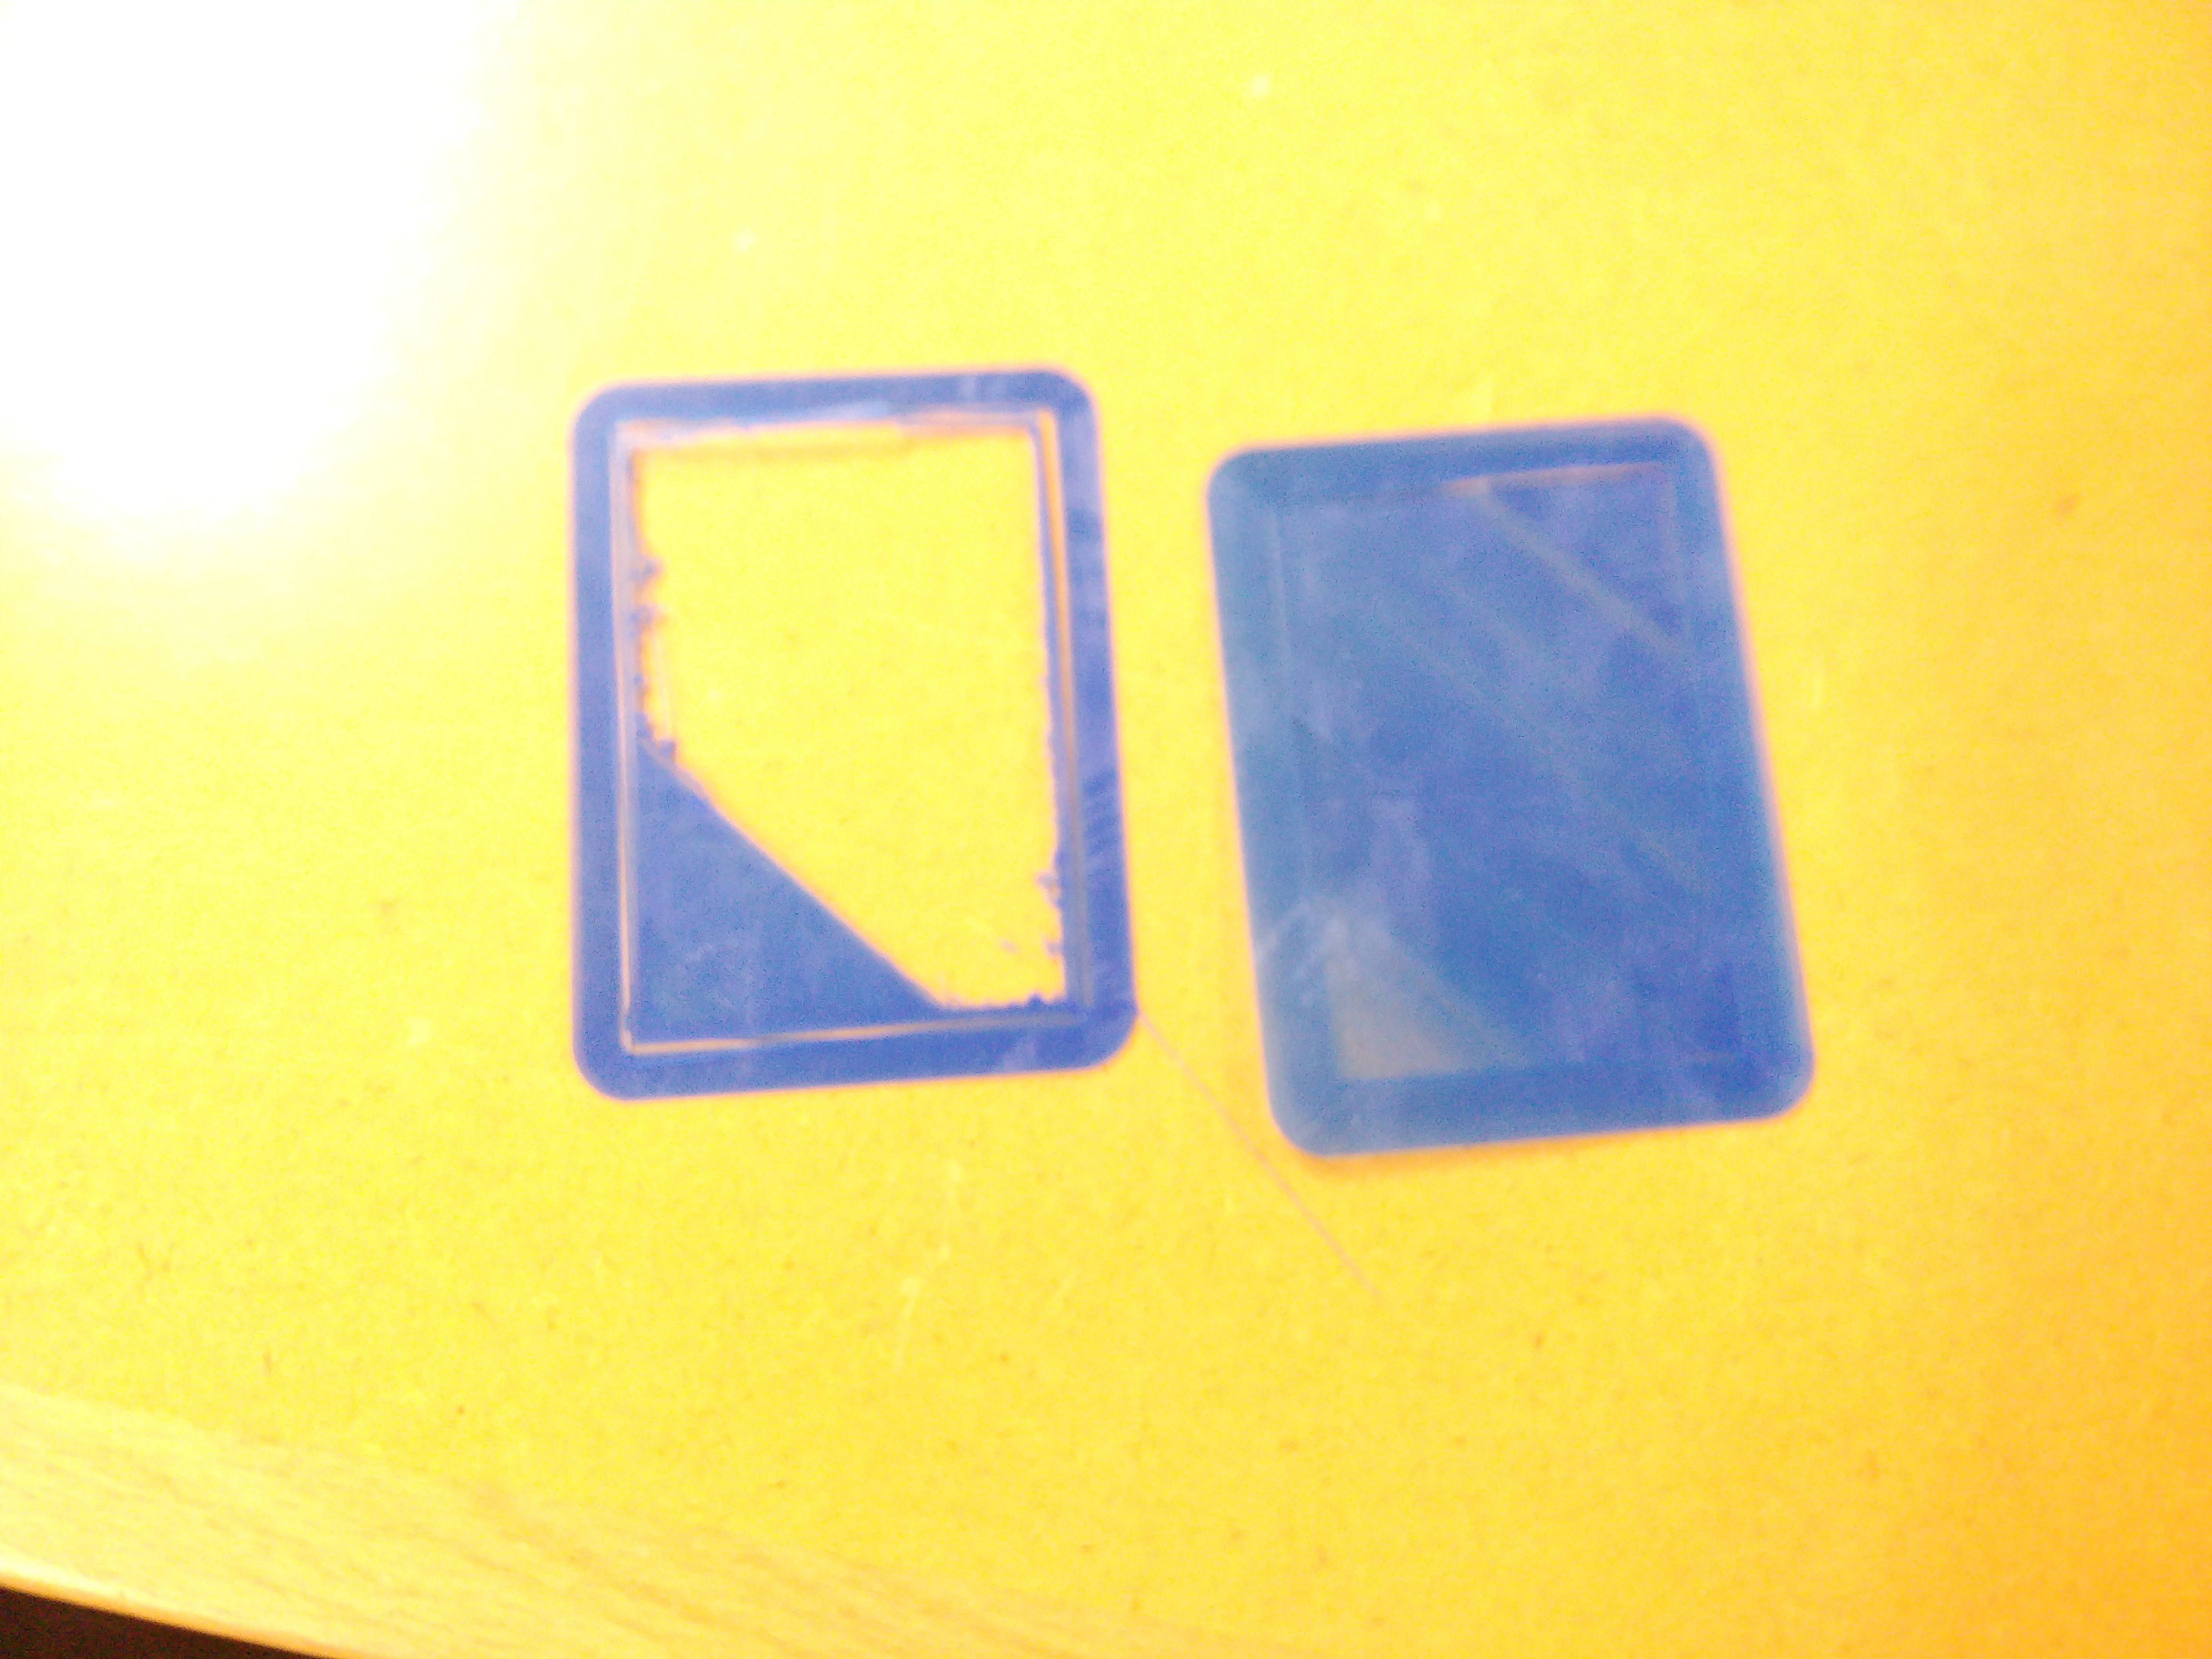
\includegraphics[width=0.3\textwidth]{../figures/Pics/failedprint.jpg}
    \caption{Failed print}
    \label{fig:failedprint}
\end{wrapfigure}

Immediately, a second print was started, but with the print moved to the second extruder.
Images of the board in the successful second print can be found in \cref{fig:case1img}.

\paragraph{Review}
The case turned out to exceed expectations in quality. The battery platform held the battery
in place surprisingly well (likely largely owing to the material of the battery casing).
The board enclosure also worked very well to secure the board. The lid also fit quite securely,
indicating the fillet worked effectively.

As expected, the pillars widened out somewhat. Despite this, the enclosure
top rail was in very good condition, especially including over the battery port - the largest
gap. Relatedly, the arch turned out to be a hindrance
and too troublesome to connect the battery wires through, and was therefore cut off instead. It
was also not centred on the battery port, due to a mistake during the design process where the
measurement was to the centre of the port, whereas the design was dimensioned to the edge of the
port only. Enough space was granted either side of the port to account for such an error,
and therefore came in use.
The cage as a whole did not prove useful, and only made removing the board from the casing more
tedious. It also was a blockage when routing the power cables, leading to no adequate way to
place them without straining them.

\subsubsection{Second case}
\paragraph{Design}
Considering the issues raised in review of the first case design, some changes were made.
The overall style of the first design was retained, with the battery and board placed
side-by-side. While resoldering the board for a flatter profile was preferred, this
was avoided to prevent any unforeseen issues in advance of the distance test and
would be revisited once testing was complete.

Extra space provided for front-facing egress of power
cables from the battery was removed from the design, amounting to \qty{204}{\mm\squared} saved.
To compensate this, a channel was cut into the battery platform for the cables to run.

A major omission from the first design was the charging port, which was now included in
this revision. The antenna hole diameter was doubled to \qty{5}{\mm}.

The board enclosure was removed, and a small fence was used to replace it.

The dimensional drawings can be found in \cref{fig:case2dwg}.

\paragraph{Manufacture}
The same manufacturing process was used as in the first case\footnote{\Cref{sec:case1manufacture}.}.
A finer print setting was used as the print was being left overnight, and therefore the greater
resolution would have no impact on turnaround time. This setting is part of Cura's default presets,
with no modifications made to fine-tune it.

\paragraph{Result}
The print turned out extremely well. Images can be found in \cref{fig:case2img}.

\paragraph{Review}
The first case was not tested with any antennae, so two issues occurred that
were not accounted for.
Despite the antennae holes being enlarged, they were still too small. This may have been due to
collapse of the layers as there were no supports (leading to oval holes that were
too small for the \gls{ufl} connector).
The board `enclosure' interfered with the \acrshort{gps} antenna wire. This can be
seen more clearly in \cref{fig:case2antennaissue}, and overall means that the board
cannot sit flat. The cable will require a relief channel of its own
like the battery wires.

This case is sufficient for testing with, even if the antennae have to be routed
out the lid. The casing with all components weighs in at \qty{55}{\g}.

There are some aspects to be mindful of when designing a third iteration.
If a flat form factor layout can be used by resoldering the boards, there is potential to
allow for a curved, and thereby more ergonomic design, however strain across the connection
must be accounted for.

Attaching to the harness was not considered at all during either of these designs, and will
be a major factor for how guiding the design. Similarly, general weatherproofing was not included.
A simple and effective method of waterproofing would be to use an o-ring as a seal, however this may
require more pressure than the plastic (in this case, \gls{pla}, which is extremely
flexible) is able to provide. This may be mitigated somewhat by using a more rigid material
(for example, \gls{abs} or \gls{pc}) and using screws to secure the lid and apply
the required amount of pressure to form an adequate seal.

Another omission was adequate antenna support. For that reason, during test a flat support
material will be used to protect the antennae. However, this will be an important 
factor with further iterations of case design, especially considering interference sources 
for the antennae being so close to a \acrshort{pcb} edge. 

\subsection{Distance test}
This test forms a crucial part of determining the suitability of the tracker to
perform its key function - tracking a remote target. It is only possible as the
culmination of every step before it.

\subsubsection{Preparation}
This test required more preparation than any performed previously.

\paragraph{Location}
Determining a suitable location for testing was of heightened importance.
The general area to perform the test was decided across the campus of the
University of Warwick. As a publicly accessible space, setting up the receiving
antenna anywhere with thoroughfare would not have been appropriate, however
easy access to the Pi to download data would be needed.

In short, the location needed to be easily accessible, but not in a location
with many people. This ruled out many of the building rooftops due to
potential safety issues and authorisation requirements. The final location
decided was room A3.27, located in the School of Engineering\footnote{
    Location on map: \cref{fig:roomlocation}.
}. This location
was sufficiently high up and had a clear view of Car Park 9 (CP204) and
Lord Bhattacharyya Way. Unfortunately, there was no logistical method with
which the antenna could be mounted outdoors from this location, and therefore
was confined to being indoors. This would severely impact the capability of the antenna.

\paragraph{Work flow}
For ease-of-access, being able to view the data log remotely would be most ideal.
It also means that, should the connection drop out, this can be noticed immediately by
viewing current incoming packets. Remote access requires some manner in which the devices
accessed appears in the `same location'. In this case, it would, in its simplest form,
require a static \acrshort{ip} assignment.
Due to the university network security requirements and address assignment protocol
(likely at best a \acrshort{dhcp} assignment from a limited pool),
there was no ideal way in which the Pi
could be assigned a static \acrshort{ip} address.

The alternative was to set the Pi and antenna up to record data, and retrieve data afterwards.
This comes with the downside that the test can no longer be dynamic. Any issues that occur can
only be investigated after the fact.

With the work flow determined, the setup has the antenna next to a window while connected to the
Pi. A laptop is then connected with an Ethernet cable to the Pi over \acrshort{ssh}.
\Cref{fig:disthardwaresetup} shows a diagram of this hardware setup.

\begin{figure}[htbp]
    \centering
    \begin{subfigure}[b]{0.65\textwidth}
        \centering
        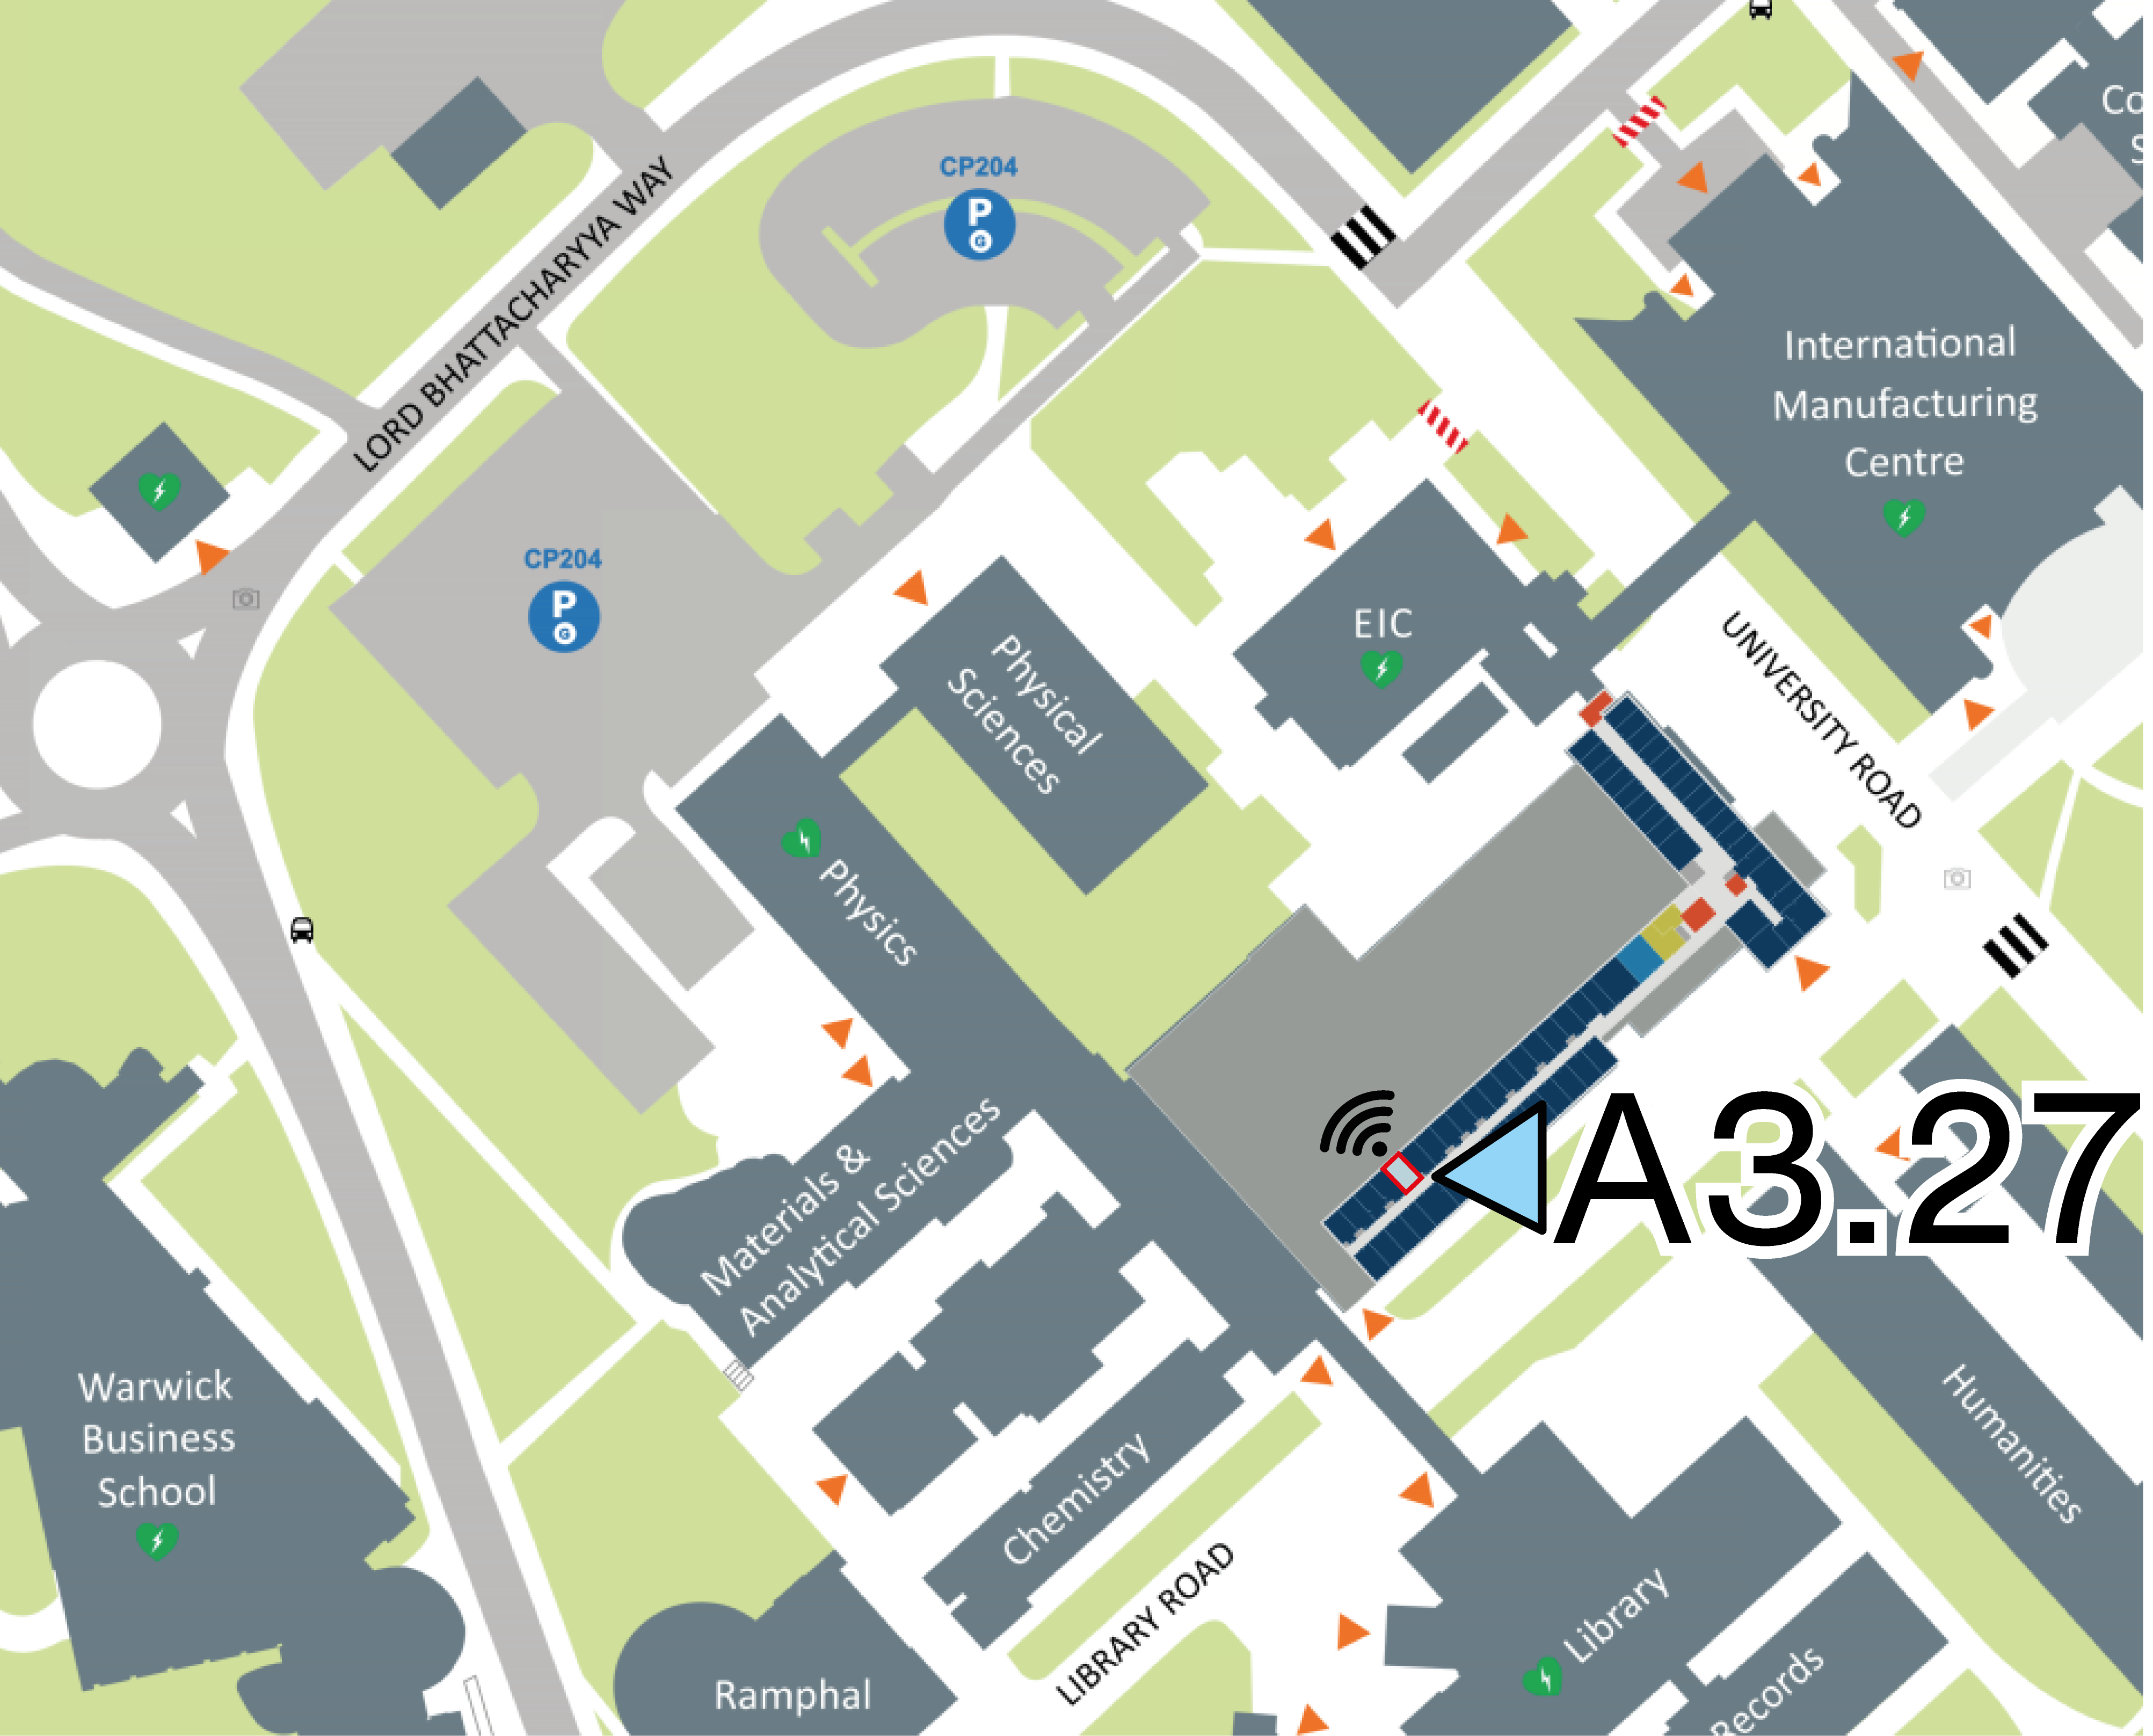
\includegraphics[height=7cm,width=\textwidth,keepaspectratio]{../figures/maps/room.png}
        \caption{A3.27 location, showing Car Park 9 (CP204)}
        \label{fig:roomlocation}
    \end{subfigure}
    \hfill
    \begin{subfigure}[b]{0.3\textwidth}
        \centering
        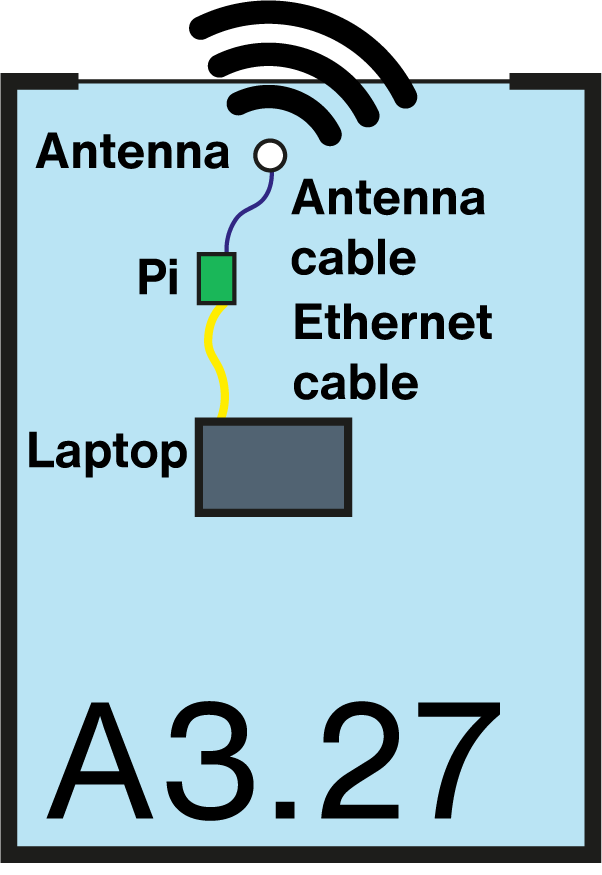
\includegraphics[height=7cm,width=\textwidth,keepaspectratio]{../figures/maps/setup.png}
        \caption{Hardware setup}
        \label{fig:disthardwaresetup}
    \end{subfigure}
    \caption{Distance test location and setup}
    \label{fig:distancesetup}
\end{figure}

\paragraph{Container}
While the transmitter now has appropriate casing, the antenna holes were too small
to run the \gls{ufl} connector through. Due to time constraints, this could not be
remedied, and instead, the antennae were exposed through the lid.
This also left them with no support, which may prove a point of failure if left unattended\footnote{
    \Cref{fig:case2antennasplay} shows how the antennae splay.
}. To secure the antennae, a scrap sheet of acrylic was used to tape them down, thereby
providing them a rigid support surface with a low chance of leading to interference.
The final result of the casing as used in testing can be seen in \cref{fig:distancerig}.

\begin{figure}[htbp]
    \centering
    \begin{subfigure}[b]{0.475\textwidth}
        \centering
        \includegraphics[height=5cm,width=\textwidth,keepaspectratio]{../figures/Pics/distancerig1.jpg}
        \caption{Overview}
    \end{subfigure}
    \hfill
    \begin{subfigure}[b]{0.475\textwidth}
        \centering
        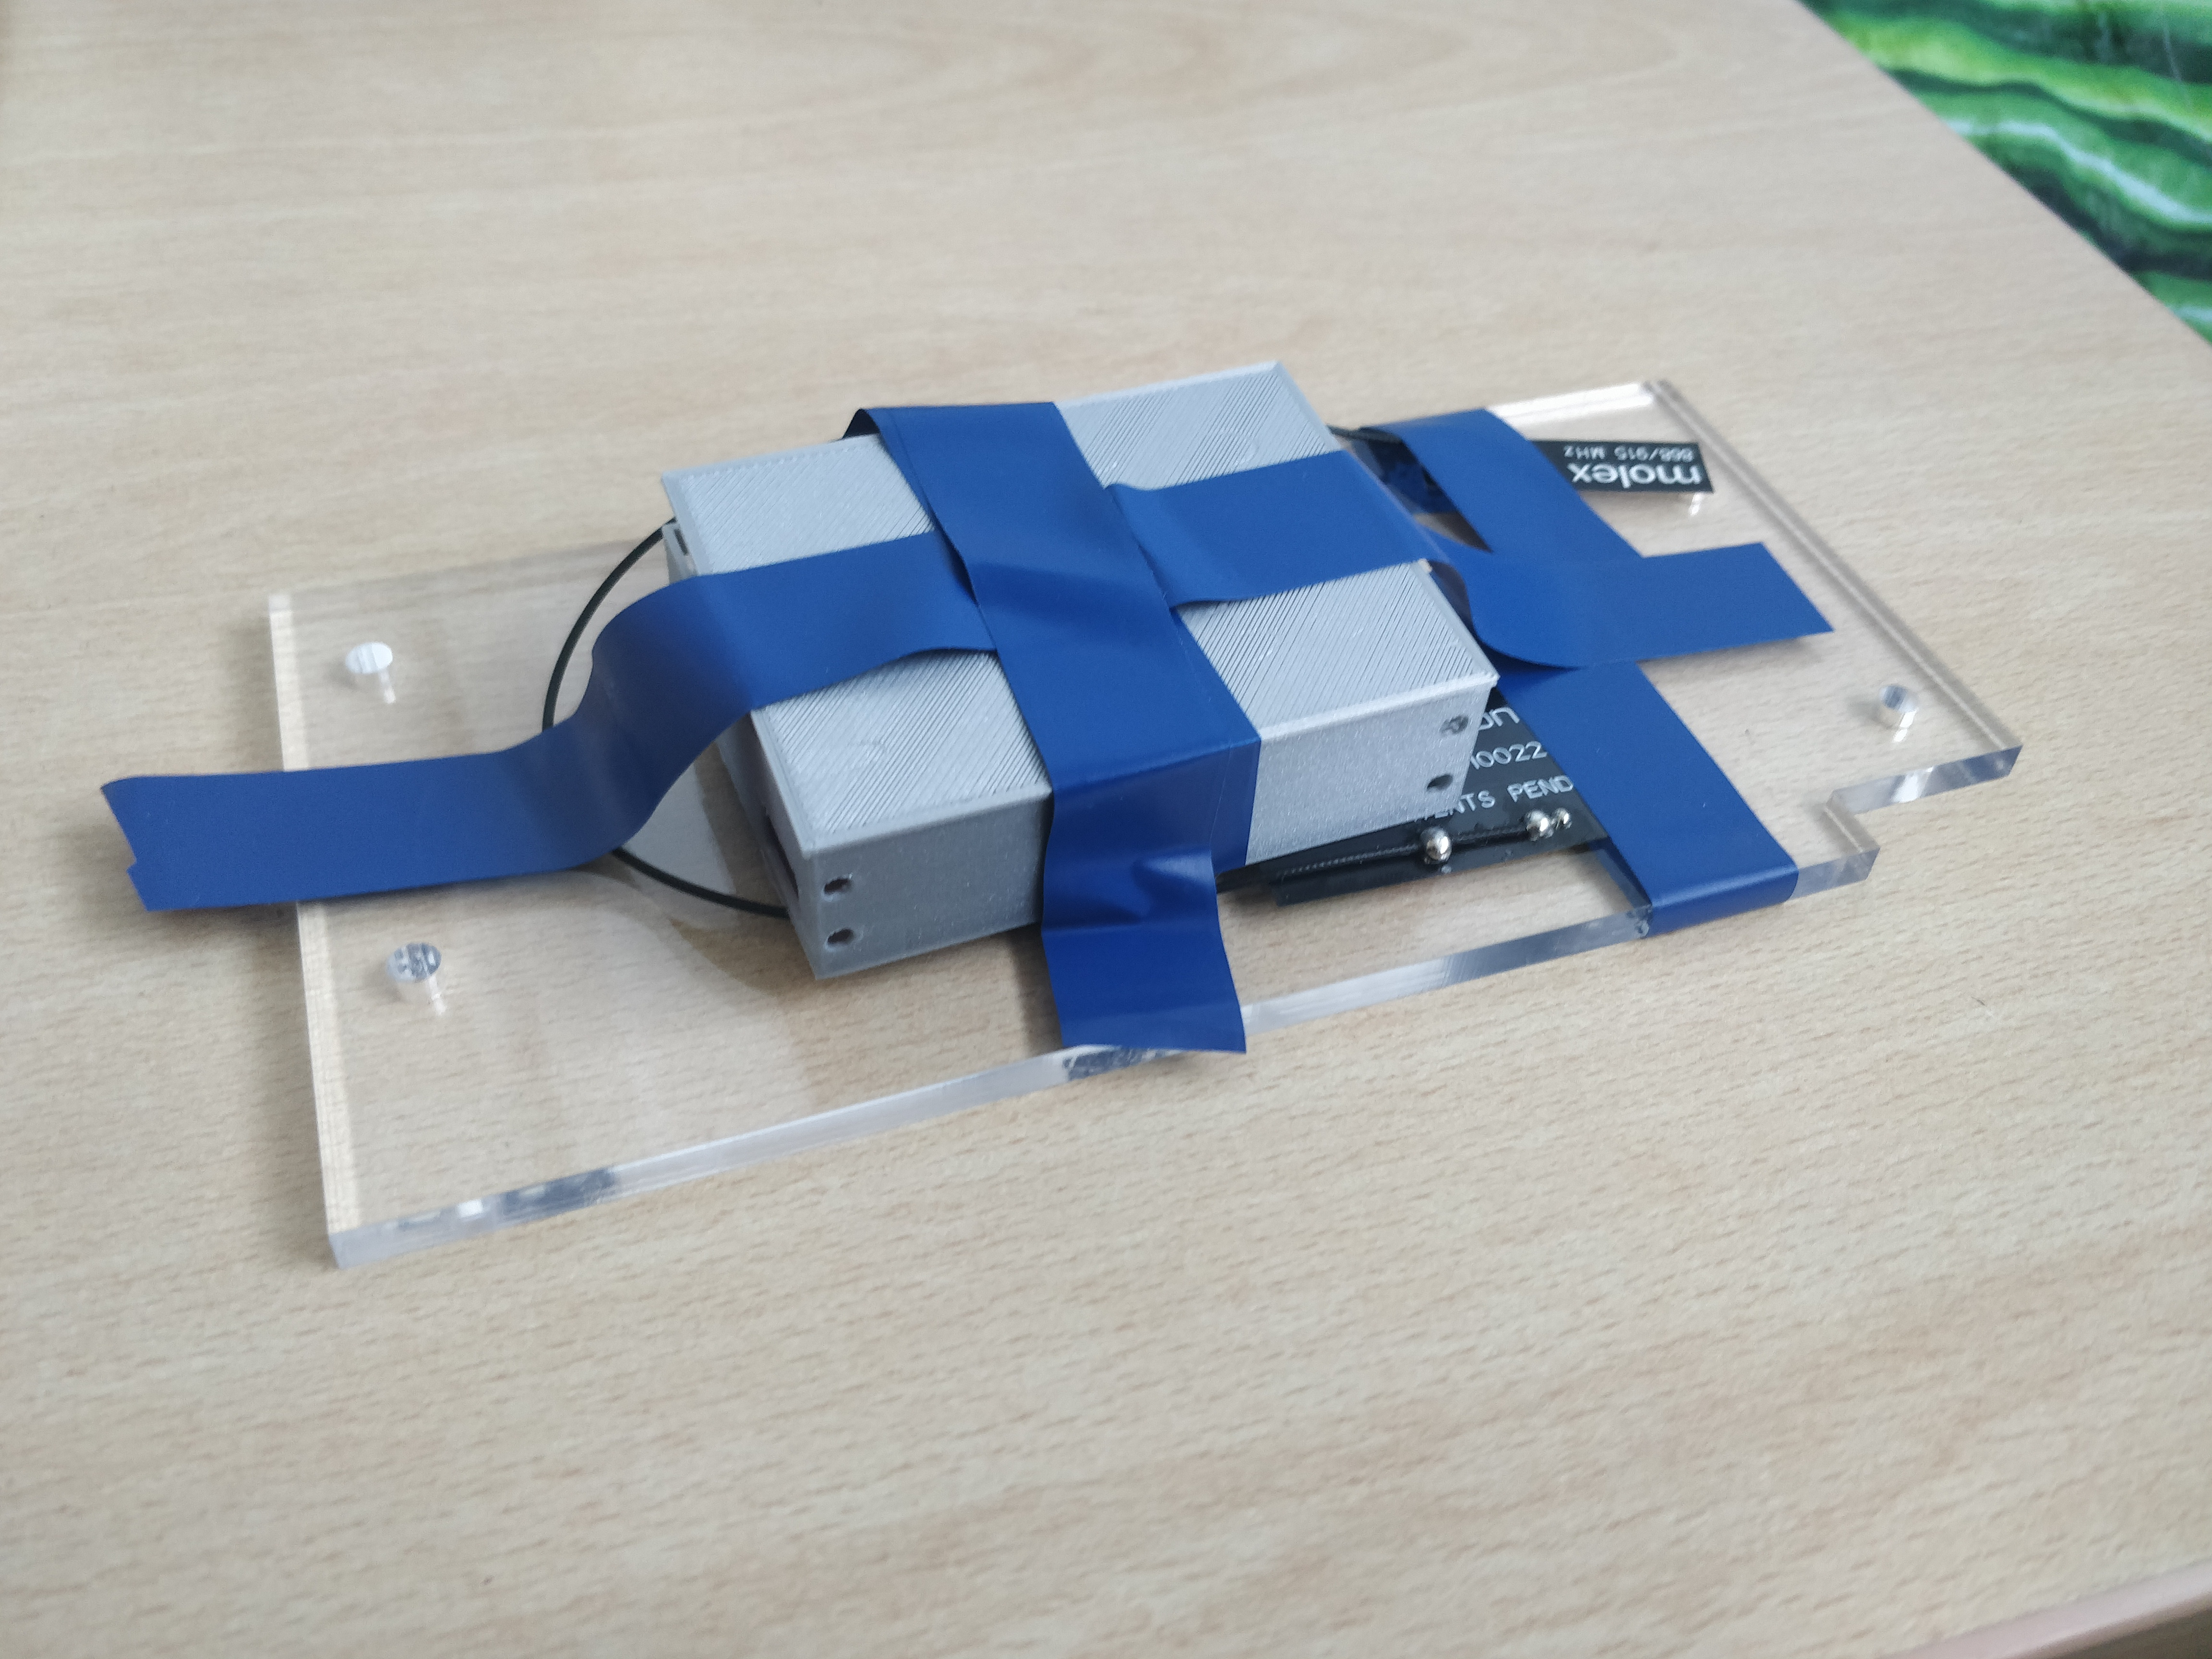
\includegraphics[height=5cm,width=\textwidth,keepaspectratio]{../figures/Pics/distancerig2.jpg}
        \caption{Angled view}
    \end{subfigure}
    \caption{Setup used for distance testing}
    \label{fig:distancerig}
\end{figure}

\paragraph{Data}

% \begin{wrapfigure}[10]{L}{0.4\textwidth}
%     \vspace{-5pt}
%     \centering
%     \includegraphics[width=0.4\textwidth]{../figures/Pics/distancedata.jpg}
%     \caption{Test data recordings}
%     \label{fig:distancedata}
% \end{wrapfigure}

An example of data recordings can be seen in \cref{fig:distancedata}. As mentioned previously\footnote{
    \Cref{sec:devgps}.
},
the output data is in a non-standard format, an example of which is given in \cref{table:invalidformat}.
In order for this data to be plotted, it needs to be converted into a standardised format, as per \cref{table:validformat}.

\begin{figure}[H]
    \centering
    \includegraphics[width=0.7\textwidth]{../figures/Pics/distancedata.jpg}
    \caption{Test data recordings}
    \label{fig:distancedata}
\end{figure}

The first step is to add direction indicators. This supports portability, but in this case will
simply be used to determine whether the direction is positive (North or East) or negative (South or West).
While the \acrshort{gps} library is able to provide directional information \cite{adafruit:gpslibrary}, 
in this instance, the output files were simply modified to include a column of the direction, 
since only locations North and West
were recorded for any tests. The modified columns in \cref{table:invalidformat} are highlighted in blue.

\parbox{.6\linewidth}{
    \begin{xltabular}{\linewidth}{|l >{\columncolor{tableh2}}cl>{\columncolor{tableh2}}c|}
        \hline
        Latitude & Direction & Longitude & Direction \\
        \hline
        5222.9409 &	N &	133.7407 &	W \\
        5222.9409 & N &	133.7407 &	W \\
        5222.9409 &	N &	133.7404 &	W \\
        \hline
        \caption[Non-standard location data format]{Non-standard location data format, with manually added columns highlighted}\label{table:invalidformat}
    \end{xltabular}
}
\quad
\parbox{.35\linewidth}{
    \begin{xltabular}{\linewidth}{|ll|}
        \hline
        Latitude & Longitude \\
        \hline
        52'22.958  &	-1'33.76  \\
        52'22.959  &	-1'33.7594 \\
        52'22.9565 &	-1'33.7566  \\
        \hline
        \caption{Desired location data format}\label{table:validformat}
    \end{xltabular}
}

With sufficient information for processing, a script was then written to convert the given format into standardised
degrees-minutes format, as per \cref{table:validformat}, the code for which can be found in \cref{script:locationformatconverter}.
The script works by processing the location columns of each
row. It performs a regular expression match to extract the minutes from the degrees, and return both in an array [lines 6-7].
It then determines the polarity by the relevant direction column, and adds the degree separator (\textquotesingle) as necessary [lines 12-14].
Finally, it writes the new format data to a new file, which can then be used for plotting.


\paragraph{Plotting}
The plotting software of choice was QGIS, a free and open-source \acrshort{gis} software package.
While QGIS has many advanced features, one of the most useful in this case is the ability to lay \acrshort{gps}
coordinates over a map. It furthermore accepts many formats of location data, including \gls{kml} markup,
which will be important as part of the verification step.

\subsubsection{Test specification}
Due to blind recording, the test is carried out with no knowledge as to how successful it is.
The transmitter was powered on by connecting the battery, and the script on the receiver\footnote{
    \Cref{pi:battery}.
} was started. The tracker was then carried around the predetermined route. At the same time,
an app based \acrshort{gps} tracker was started, which records location data independently.
When the route was complete, the data was downloaded for later processing and comparison
to the externally recorded data.

\paragraph{Risks}
Inclement weather may cause a problem for the circuitry, as the casing is not 
waterproofed. 
Otherwise, only typical precautions when travelling outdoors near roads are 
necessary. 

\subsubsection{Test one}
The route was determined to include walking behind the School of Engineering and around
Lord Bhattacharyya Way while holder the transmitter.
This route covered a maximum straight line distance of \qty{175}{\m}
and involved parts with direct line of sight to the receiver, and large sources of interference
in other areas (e.g. buildings, antennae, girders, etc).

This test was performed with perhaps what could be considered the worst possible conditions,
and success from hereupon would determine whether an altered setup was required. To check suitability,
after the test was run, the data logs would be checked to see whether there was consistent location
information. If so, a second test at a greater distance would be performed. If not, the
setup would be revisited.

\paragraph{Results}
After the test was performed, the logs appeared to indicate successful transmission, although
this could not be analysed at the time. As such, a second test at a much greater distance was
performed immediately afterwards.

\Cref{fig:dtest1} shows the recorded points in red\footnote{
    Data sample in \cref{table:distancetest1}.
} and the externally recorded route in blue\footnote{
    Data sample in \cref{kmltest1}.
}
after processing. As can be seen, the results are well-matched. Despite the extremely poor
testing conditions, the tracker operated surprisingly well.

\begin{figure}[htbp]
    \centering
    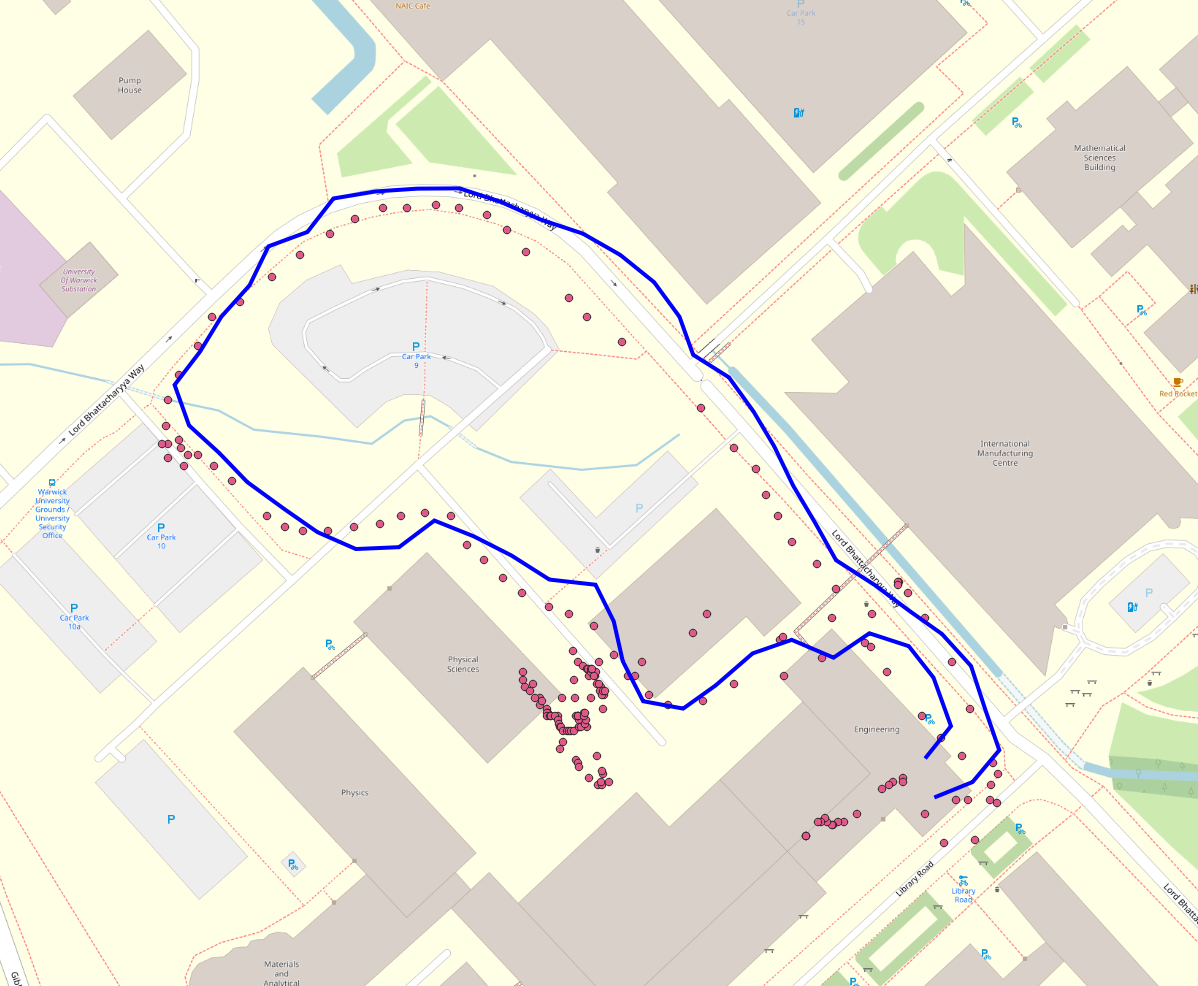
\includegraphics[height=10cm]{../figures/maps/test1 overlay.png}
    \caption[Distance test one overlay]{Location recordings with route overlay}
    \label{fig:dtest1}
\end{figure}

% \begin{wrapfigure}{R}{0.7\textwidth}
%     \vspace{-5pt}
%     \centering
%     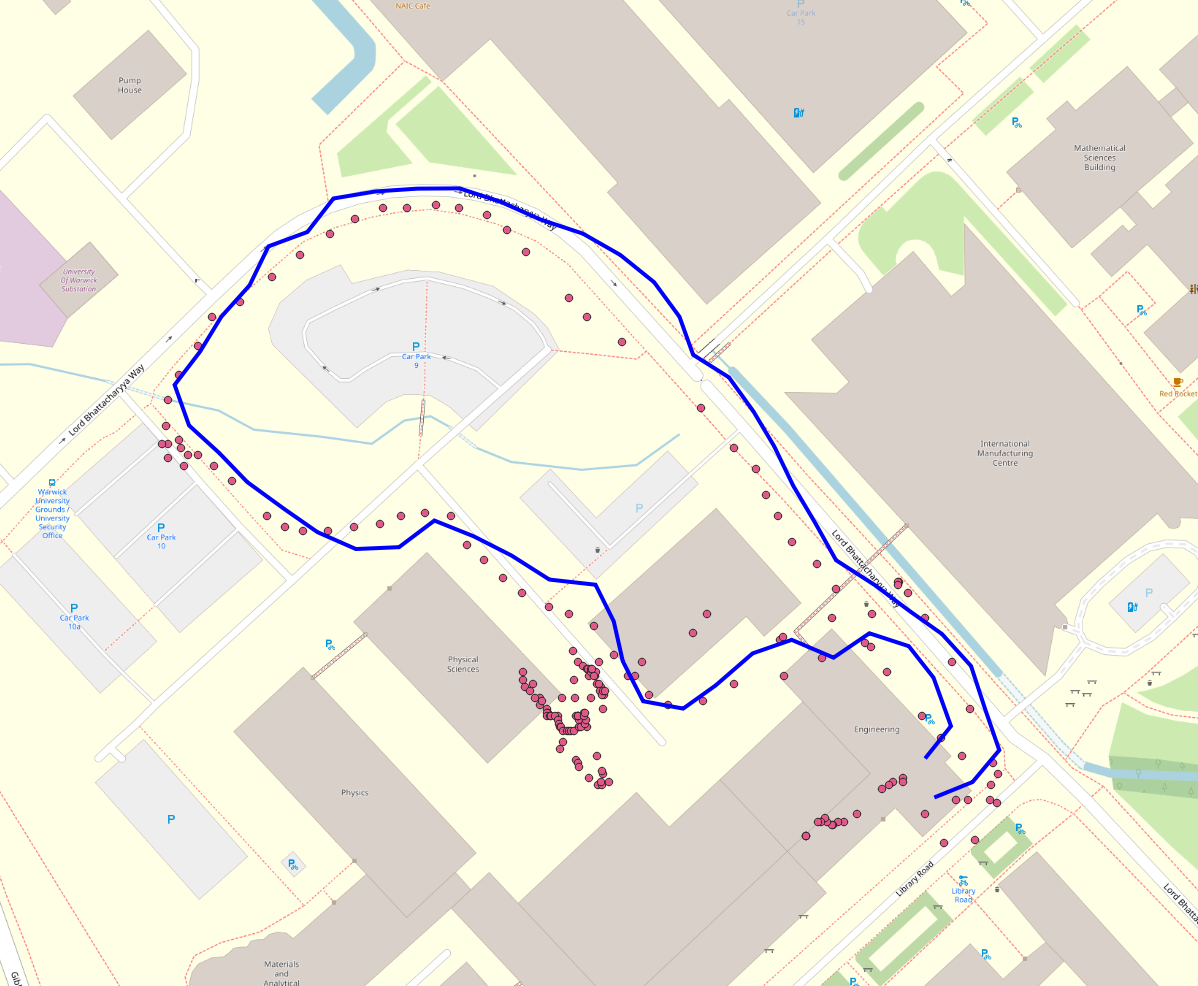
\includegraphics[width=0.65\textwidth]{../figures/maps/test1 overlay.png}
%     \caption[Distance test one overlay]{Location recordings with route overlay}
%     \label{fig:dtest1}
% \end{wrapfigure}

A cluster of points next
to Physical Sciences, is likely points recorded in A3.27, but offset due to inaccuracies
in location while indoors. A smaller cluster next to Car Park 10 is due to a slightly longer
period of time spent in that location.

There are no noticeable errors or omissions present. The location data recorded by the
tracker also appears to be more accurate to the precise route followed than is indicated by
app-based tracker.

\subsubsection{Test two}
Given the apparent positive results of the first test, the second test 
was devised to cover a much greater distance. In this case, the route consisted 
of Kirby Corner Rd. and Charter Ave. in a large triangle, with the greatest distance 
\qty{1.2}{\km} away. This test was devised in this manner to cover the most extreme 
capabilities of the tracker, since it is impossible to determine live whether a 
range is too great. 

The route includes a number of points that would be in `line of sight' (were it not for foliage),
in addition to areas of dense foliage and building obstructions. 

Due to the distances involved, the mode of transportation chosen was bicycle. This would 
at least affect the distance between reported locations. It is also possible that 
transmissions would be affected due to the speed. Furthermore, the tracker could no longer
be held and would have to be carried in a pocket, which may affect transmission capabilities. 

\paragraph{Results}
After testing, the logs appeared to have much fewer records than expected\footnote{
    Data sample in \cref{table:distancetest2}.
}. Furthermore, the 
app-based tracker failed to work. In \cref{fig:dtest2}, the travelled route was drawn on afterwards.
Noticeably, there are far fewer points plotted, and of that, the furthest was \qty{436}{\m} away with 
the majority of the route missing. 
This position did not have clear sight, however it was a position with the `least' obstruction
at that distance. The points were spaced out a greater distance,  which was expected. 

\begin{figure}[htb!]
    \centering
    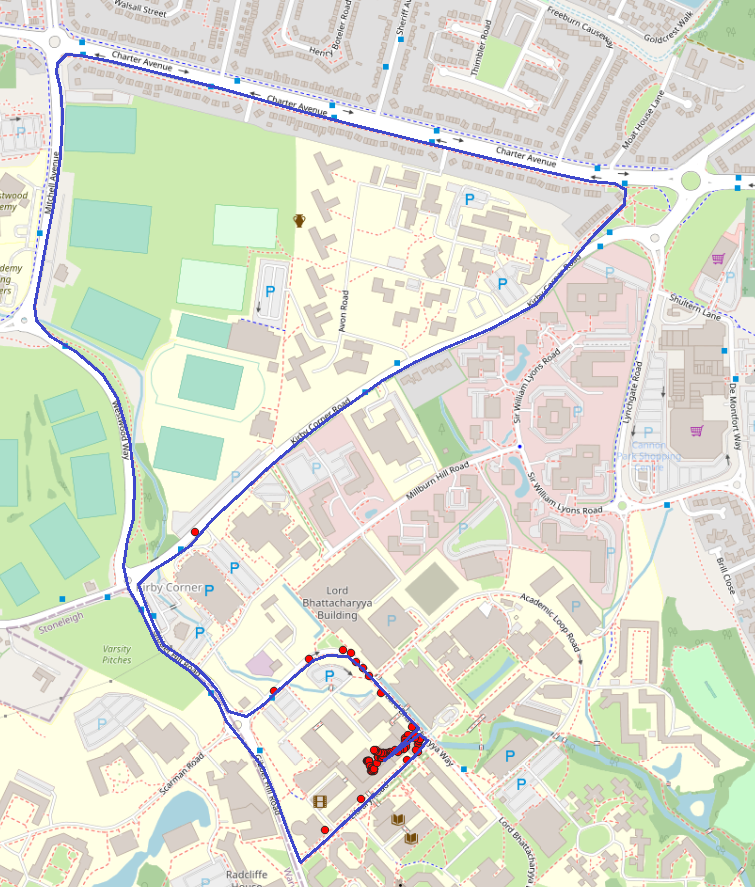
\includegraphics[height=12cm]{../figures/maps/test2 overlay.png}
    \caption[Distance test two overlay]{Location recordings with route overlay}
    \label{fig:dtest2}
\end{figure}

% \begin{wrapfigure}{R}{0.7\textwidth}
%     \vspace{-5pt}
%     \centering
%     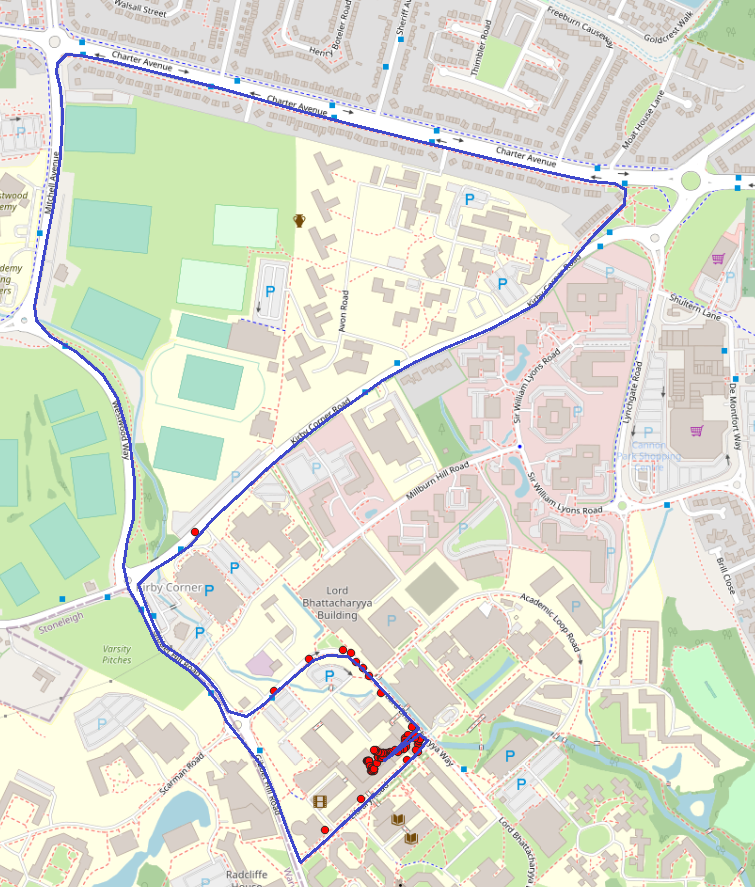
\includegraphics[width=0.65\textwidth]{../figures/maps/test2 overlay.png}
%     \caption[Distance test two overlay]{Location recordings with route overlay}
%     \label{fig:dtest2}
% \end{wrapfigure}

Focusing on the points recorded on Lord Bhattacharyya Way and Library Rd.,
assuming these points were sequential (\qty{5}{\s}) transmissions, this indicates an 
approximate travel speed of \qty{40}{\km\per\hour} to \qty{55}{\km\per\hour}. This 
is practically impossible to be the case, therefore suggesting there were either missing points
during transmission, or the recorded location is not precise enough to calculate 
the speed from (where it is `large'). 

Due to insufficient reporting, it is impossible to determine whether \acrshort{gps} location was
lost at any point. Periodic checks on the device suggest this did not happen\footnote{
    While searching for a fix, the \acrshort{gps} module will blink its \acrshort{led} every second.
    If a fix is found, this will increase to every fifteen, and can be used to easily indicate if 
    there is a fix \cite{adafruit:gps}. 
}.

\subsubsection{Comments}

Overall, the conclusion to be drawn from this suite of tests is that the tracker is very clearly 
viable for its purposes, however requires some points of refinement. 

Test one went extremely well, with no particular major issues identified. It is most useful 
in comparison to test two, where almost all the route was not sufficiently tracked. 
This difference likely comes down to two things - the distance travelled being obviously much greater, 
and the tracker being held in a pocket. 

Regarding distance, the area overlapped by both tests was reported on with acceptable clarity. 
This suggests the greatest issue was simply difficulty transmitting over range, or the increasing
number of interference sources as distance (and perhaps speed of travel) increased. 

It is particularly noteworthy that the test conditions were the poorest possible, possible aside 
from the addition of rain. The receiving antenna was placed indoors where it would preferably
be outdoors, and the tracker was held in a pocket where it would also be preferably exposed. 
The general area was heavily built with many sources of interference, inexhaustibly 
including trees, buildings, and metal structures. While elevated, the surrounding area was heavily built
up, with only a small area of space between buildings where the ground (and thereby, tracker) could be seen\footnote{
    This area is where Car Park 9 is located, however it is still has much foliage in the way. 
}.  
The location in particular, a university campus, suggests that there was also a 
higher likelihood of \acrshort{rf} interference sources.  

Finally, the data, while indicative of function, is far from complete. Performing more tests, especially in different 
conditions, to accurately determine the limits of the tracker conclusively would be advised. 
The information gleaned from these tests is meaningful, yet incomplete in thoroughness. 



